% -*- latex -*-
%%%%%%%%%%%%%%%%%%%%%%%%%%%%%%%%%%%%%%%%%%%%%%%%%%%%%%%%%%%%%%%%
%%%%%%%%%%%%%%%%%%%%%%%%%%%%%%%%%%%%%%%%%%%%%%%%%%%%%%%%%%%%%%%%
%%%%
%%%% This text file is part of the lecture slides for
%%%% `Parallel Computing'
%%%% by Victor Eijkhout, copyright 2012-2020
%%%%
%%%% PTP-slides.tex: slides about point-to-point communication
%%%%
%%%%%%%%%%%%%%%%%%%%%%%%%%%%%%%%%%%%%%%%%%%%%%%%%%%%%%%%%%%%%%%%
%%%%%%%%%%%%%%%%%%%%%%%%%%%%%%%%%%%%%%%%%%%%%%%%%%%%%%%%%%%%%%%%

\begin{frame}[containsverbatim]{Overview}
  This section concerns direct communication
  between two processes. Discussion of distributed work, deadlock and
  other parallel phenomena.

  Commands learned:
  \begin{itemize}
  \item
    \indexmpishow{MPI_Send}, \indexmpishow{MPI_Recv},
    \indexmpishow{MPI_Sendrecv}, \indexmpishow{MPI_Isend}, \indexmpishow{MPI_Irecv}
  \item \indexmpishow{MPI_Wait...}
  \item Mention of \indexmpishow{MPI_Test},
    \indexmpishow{MPI_Bsend}\lstinline{/Ssend/Rsend}.
  \end{itemize}
\end{frame}

\sectionframe{Point-to-point communication}

\begin{frame}\frametitle{MPI point-to-point mechanism}
  \begin{itemize}
  \item Two-sided communication
  \item Matched send and receive calls
  \item One process sends to a specific other process
  \item Other process does a specific receive.
  \end{itemize}
\end{frame}

\setbox1=\vbox{
  Process~A executes the code
\lstset{language=C}
\begin{lstlisting}
MPI_Send( /* to: */ B ..... );
MPI_Recv( /* from: */ B ... );
\end{lstlisting}
Process~B executes
\begin{lstlisting}
MPI_Recv( /* from: */ A ... );
MPI_Send( /* to: */ A ..... );
\end{lstlisting}
}

\begin{frame}\frametitle{Ping-pong}
  A sends to B, B sends back to A

  \only<1>{What is the code for A? For B?}
  \only<2>{\medskip \box1}
\end{frame}

\begin{frame}[containsverbatim]\frametitle{Ping-pong in MPI}
Remember SPMD:
\lstset{language=C}
\begin{lstlisting}
if ( /* I am process A */ ) {
  MPI_Send( /* to: */ B ..... );
  MPI_Recv( /* from: */ B ... );
} else if ( /* I am process B */ ) {
  MPI_Recv( /* from: */ A ... );
  MPI_Send( /* to: */ A ..... );
}
\end{lstlisting}
\end{frame}

\protoslide{MPI_Send}
\protoslide{MPI_Recv}

\begin{frame}[containsverbatim]\frametitle{Status object}
  \begin{itemize}
  \item Receive call can have various wildcards:\\
    \indexmpishow{MPI_ANY_SOURCE}, \indexmpishow{MPI_ANY_TAG}
  \item Receive buffer size is actually upper bound, not exact:
  \item Use status object to retrieve actual description of the message
  \item Use \indexmpishow{MPI_STATUS_IGNORE} if the above does not apply
  \end{itemize}
\end{frame}

\begin{exerciseframe}[pingpong]
  \input ex:pingpong
\end{exerciseframe}

\protoslide{MPI_Wtime}

\sectionframe{Distributed data}

\begin{frame}[containsverbatim]\frametitle{Distributed data}
  Distributed array: each process stores disjoint local part
  
  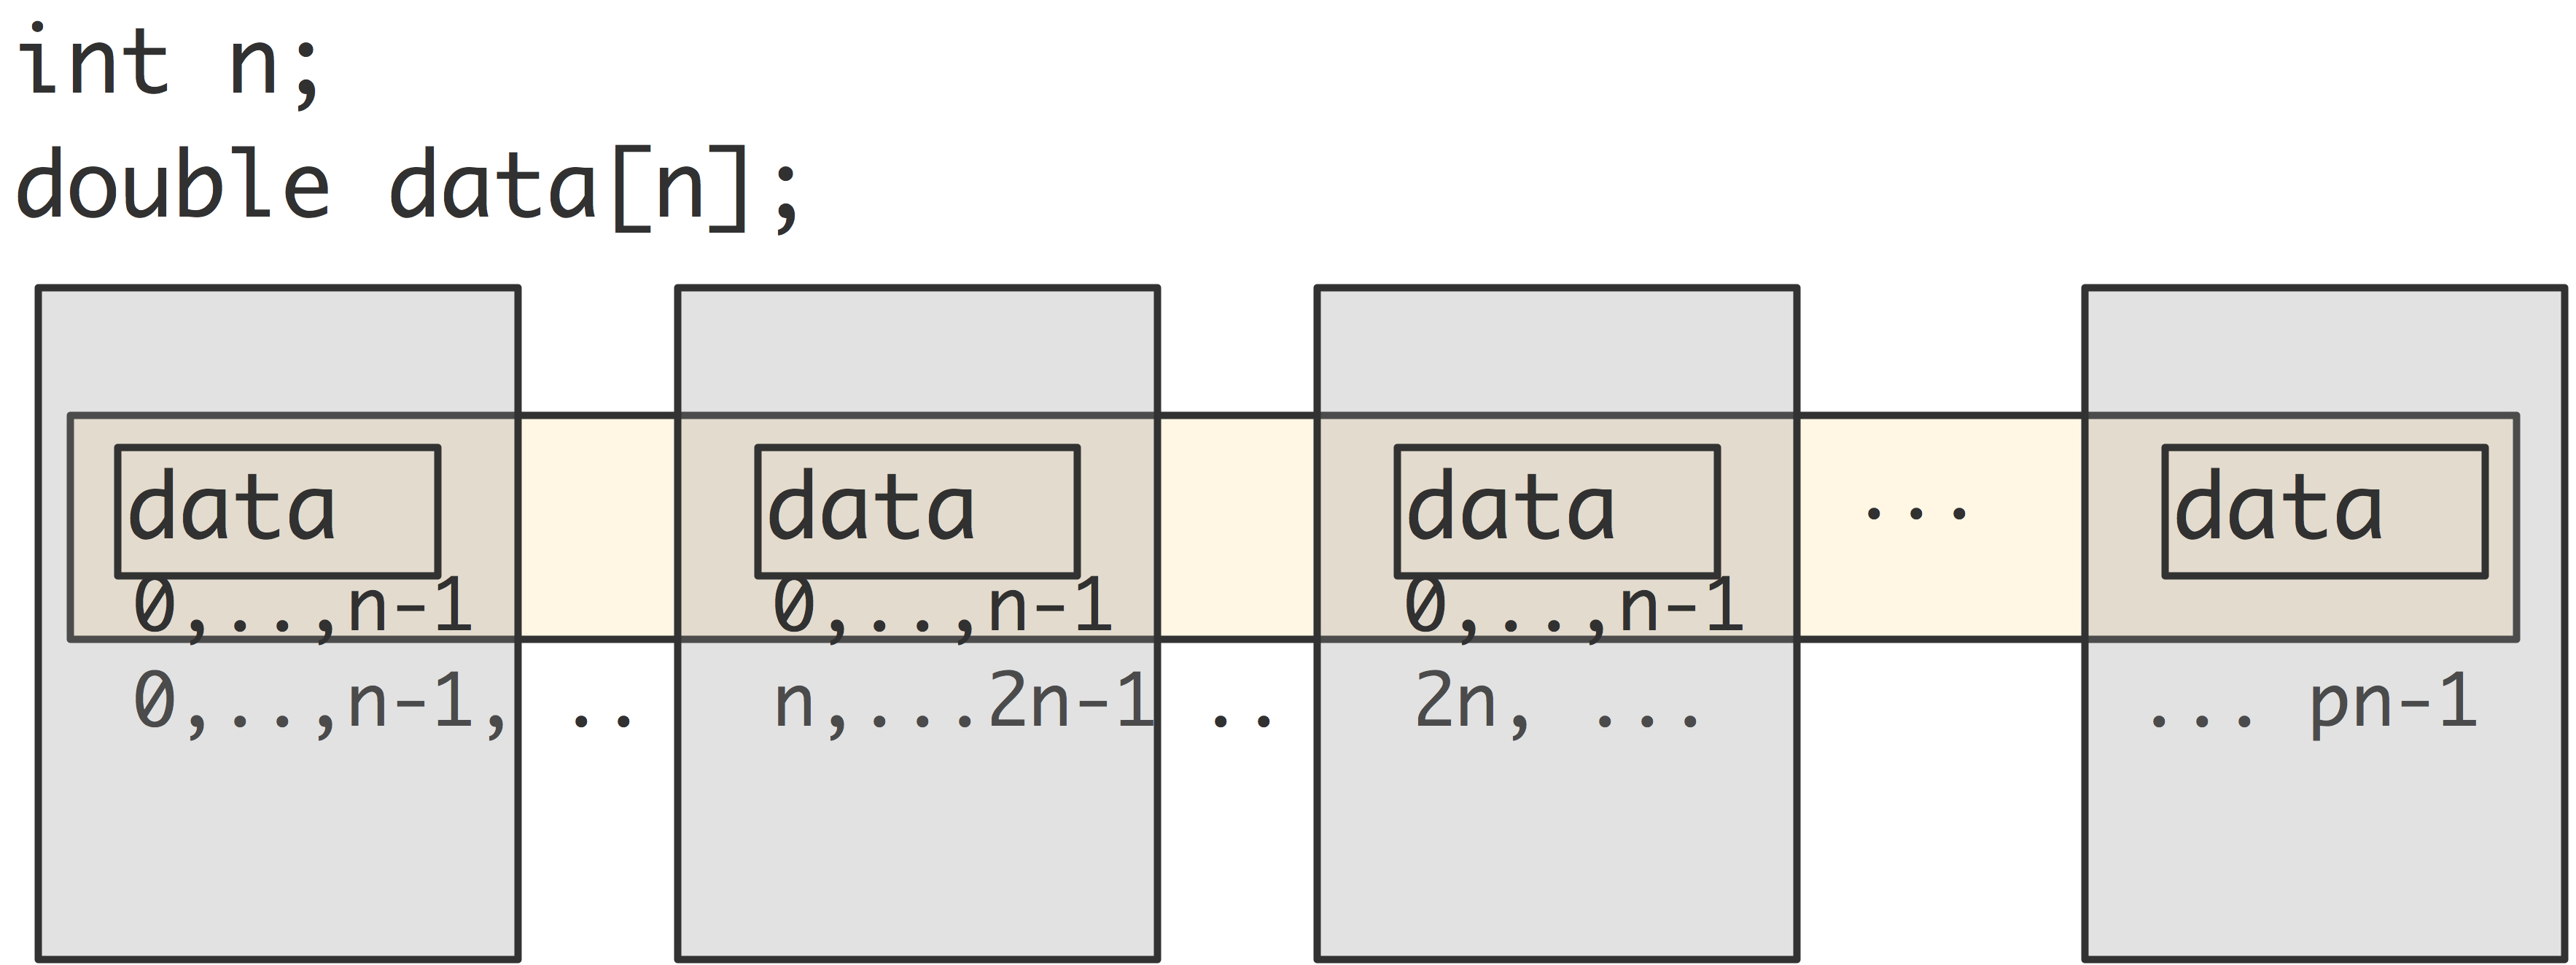
\includegraphics[scale=.09]{mpi-array}

  Local numbering $0,\ldots,n_{\mathrm{local}}$;\\
  global numbering is `in your mind'.
\end{frame}

\begin{frame}[containsverbatim]\frametitle{Local and global indexing}
  Every local array starts at 0 (Fortran:~1);\\
  you have to translate that yourself to global numbering:
\lstset{language=C}
\begin{lstlisting}
int myfirst = .....;
for (int ilocal=0; ilocal<nlocal; ilocal++) {
   int iglobal = myfirst+ilocal;
   array[ilocal] = f(iglobal);
}  
\end{lstlisting}
\end{frame}

\begin{frame}[containsverbatim]\frametitle{Load balancing}
If the distributed array is not perfectly divisible:
\lstset{language=C}
\begin{lstlisting}
int Nglobal, // is something large
    Nlocal = Nglobal/nprocs,
    excess = Nglobal%nprocs;
if (procno==nprocs-1) 
  Nlocal += excess;
\end{lstlisting}
This gives a load balancing problem. Better solution?
\end{frame}

\begin{frame}\frametitle{(for future reference)}
Let
\[ f(i)=\lfloor iN/p\rfloor \]
and give process $i$ the points $f(i)$ up to $f(i+1)$. \\
Result:
\[ \lfloor N/p\rfloor \leq f(i+1)-f(i)\leq \lceil N/p\rceil \]
\end{frame}

\begin{frame}[containsverbatim]\frametitle{Inner product calculation}
  Given vectors $x,y$:
  \[ x^ty = \sum_{i=0}^{N-1} x_iy_i \]
  Start out with a distributed vector.
  \begin{itemize}
  \item Wrong way: collect the vector on one process and evaluate.
  \item Right way: compute local part, then collect local sums.
  \end{itemize}
\lstset{language=C}
\begin{lstlisting}
local_inprod = 0;
for (i=0; i<localsize; i++)
  local_inprod += x[i]*y[i];
MPI_Allreduce( &local_inprod, &global_inprod, 1,MPI_DOUBLE ... ) 
\end{lstlisting}
\end{frame}

\begin{comment}
  \begin{optexerciseframe}[inprod]
    \input ex:inproduct
  \end{optexerciseframe}
\end{comment}

\begin{optexerciseframe}
  \input ex:fft-vector
\end{optexerciseframe}

\sectionframe{Local information exchange}

\begin{frame}{Motivation}
  Partial differential equations:
  \[
    \hbox{$-\Delta u = -u_{xx}(\bar x)-u_{yy}(\bar x)=f(\bar x)$ for
      $\bar x\in\Omega=[0,1]^2$ 
      with $u(\bar x)=u_0$ on $\delta\Omega$.}
    \]
  Simple case:
  \[ -u_{xx}=f(x). \]
  Finite difference approximation:
  \[ \frac{2u(x)-u(x+h)-u(x-h)}{h^2}=f(x,u(x),u'(x))+O(h^2), \]
\end{frame}

\begin{frame}{Motivation (continued)}
  Equations
  \[
  \begin{cases}
    -u_{i-1} + 2u_i - u_{i+1} = h^2f(x_i)&1<i<n \\
    2u_1-u_2=h^2f(x_1)+u_0\\
    2u_n-u_{n-1}=h^2f(x_{n})+u_{n+1}.
  \end{cases}
  \]
  \begin{equation}
    \begin{pmatrix}
      2&-1&&\emptyset\\ -1&2&-1\\ \emptyset&\ddots&\ddots&\ddots
    \end{pmatrix}
    \begin{pmatrix}
      u_1\\ u_2\\ \vdots
    \end{pmatrix}
    =
    \begin{pmatrix}
      h^2f_1+u_0\\ h^2f_2\\ \vdots
    \end{pmatrix}
    \label{eq:1d2nd-matrix-vector}
  \end{equation}
  So we are interested in sparse/banded matrices.
\end{frame}

\begin{frame}{Matrix vector product}
  Most common operation: matrix vector product
  \[ y\leftarrow Ax,\qquad
  A = \begin{pmatrix}
      2&-1\\ -1&2&-1\\ &\ddots&\ddots&\ddots
    \end{pmatrix}
    \begin{pmatrix}
      u_1\\ u_2\\ \vdots
    \end{pmatrix}
  \]
  \begin{itemize}
  \item Component operation: $y_i=2x_i-x_{i-1}-x_{i+1}$
  \item Parallel execution: each process has range of $i$-coordinates
  \item So we need a point-to-point mechanism
  \end{itemize}  
\end{frame}

\begin{frame}[containsverbatim]\frametitle{Operating on distributed data}
Array of numbers $x_i\colon i=0,\ldots,N$\\
compute \[ y_i= -x_{i-1}+2x_i-x_{i+1} \colon i=1,\ldots,N-1 \]
'owner computes'\\
This leads to communication:

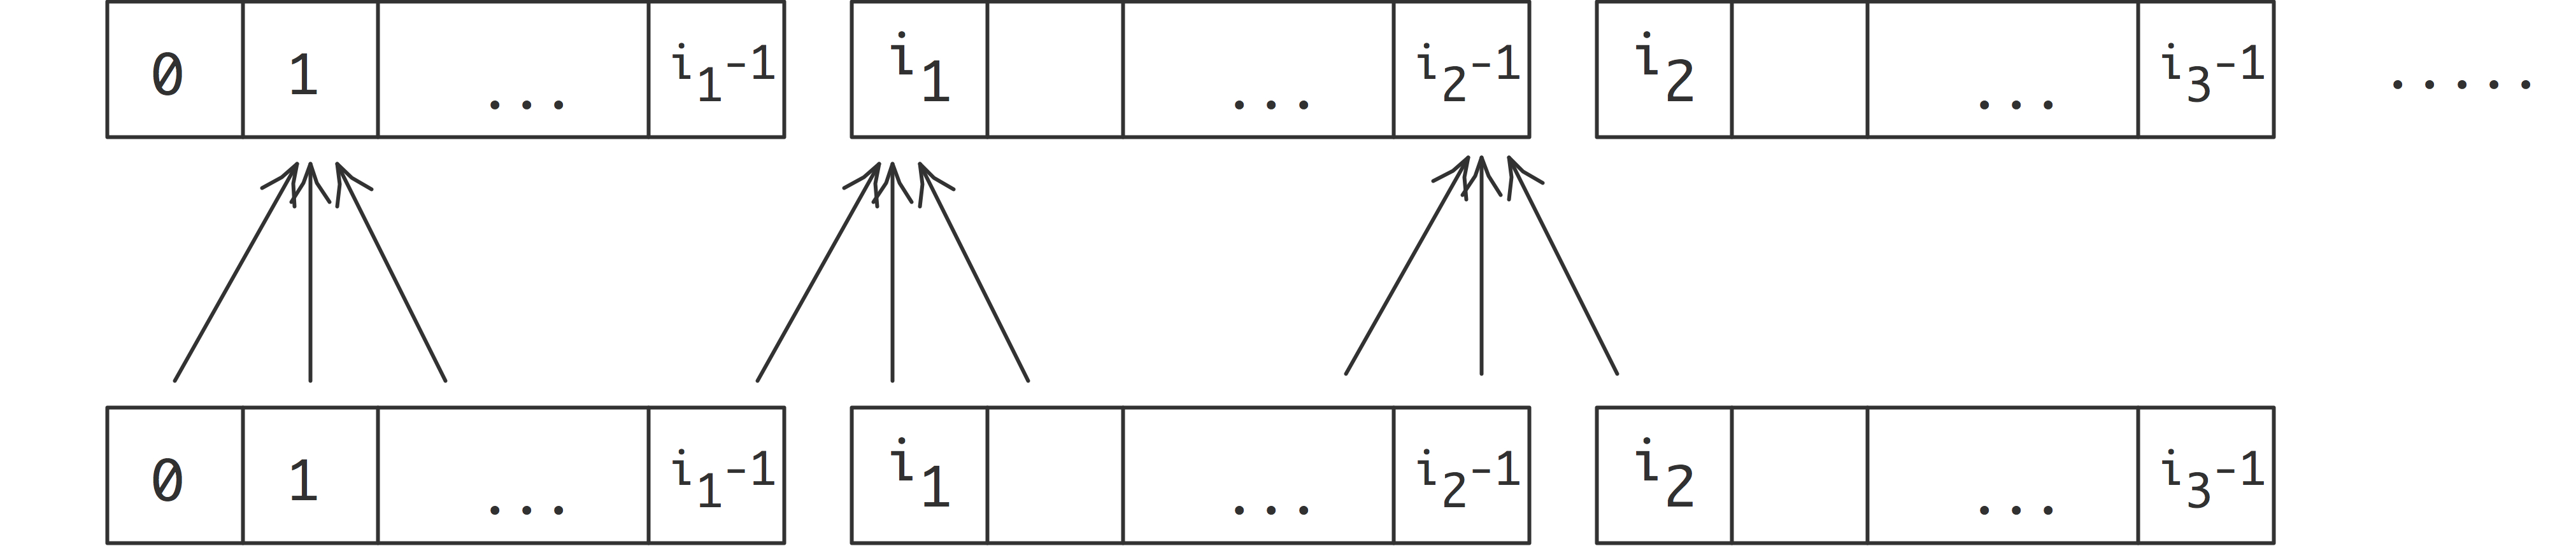
\includegraphics[scale=.09]{threepoint}

so we need a point-to-point mechanism.
\end{frame}

\sectionframe{Blocking communication}

\begin{frame}[containsverbatim]\frametitle{Blocking send/recv}
\indexmpishow{MPI_Send} and \indexmpishow{MPI_Recv} are \emph{blocking} operations:
\begin{itemize}
\item The process waits (`blocks') until the operation is concluded.
\item A send can not complete until the receive executes.
\end{itemize}
\hbox{
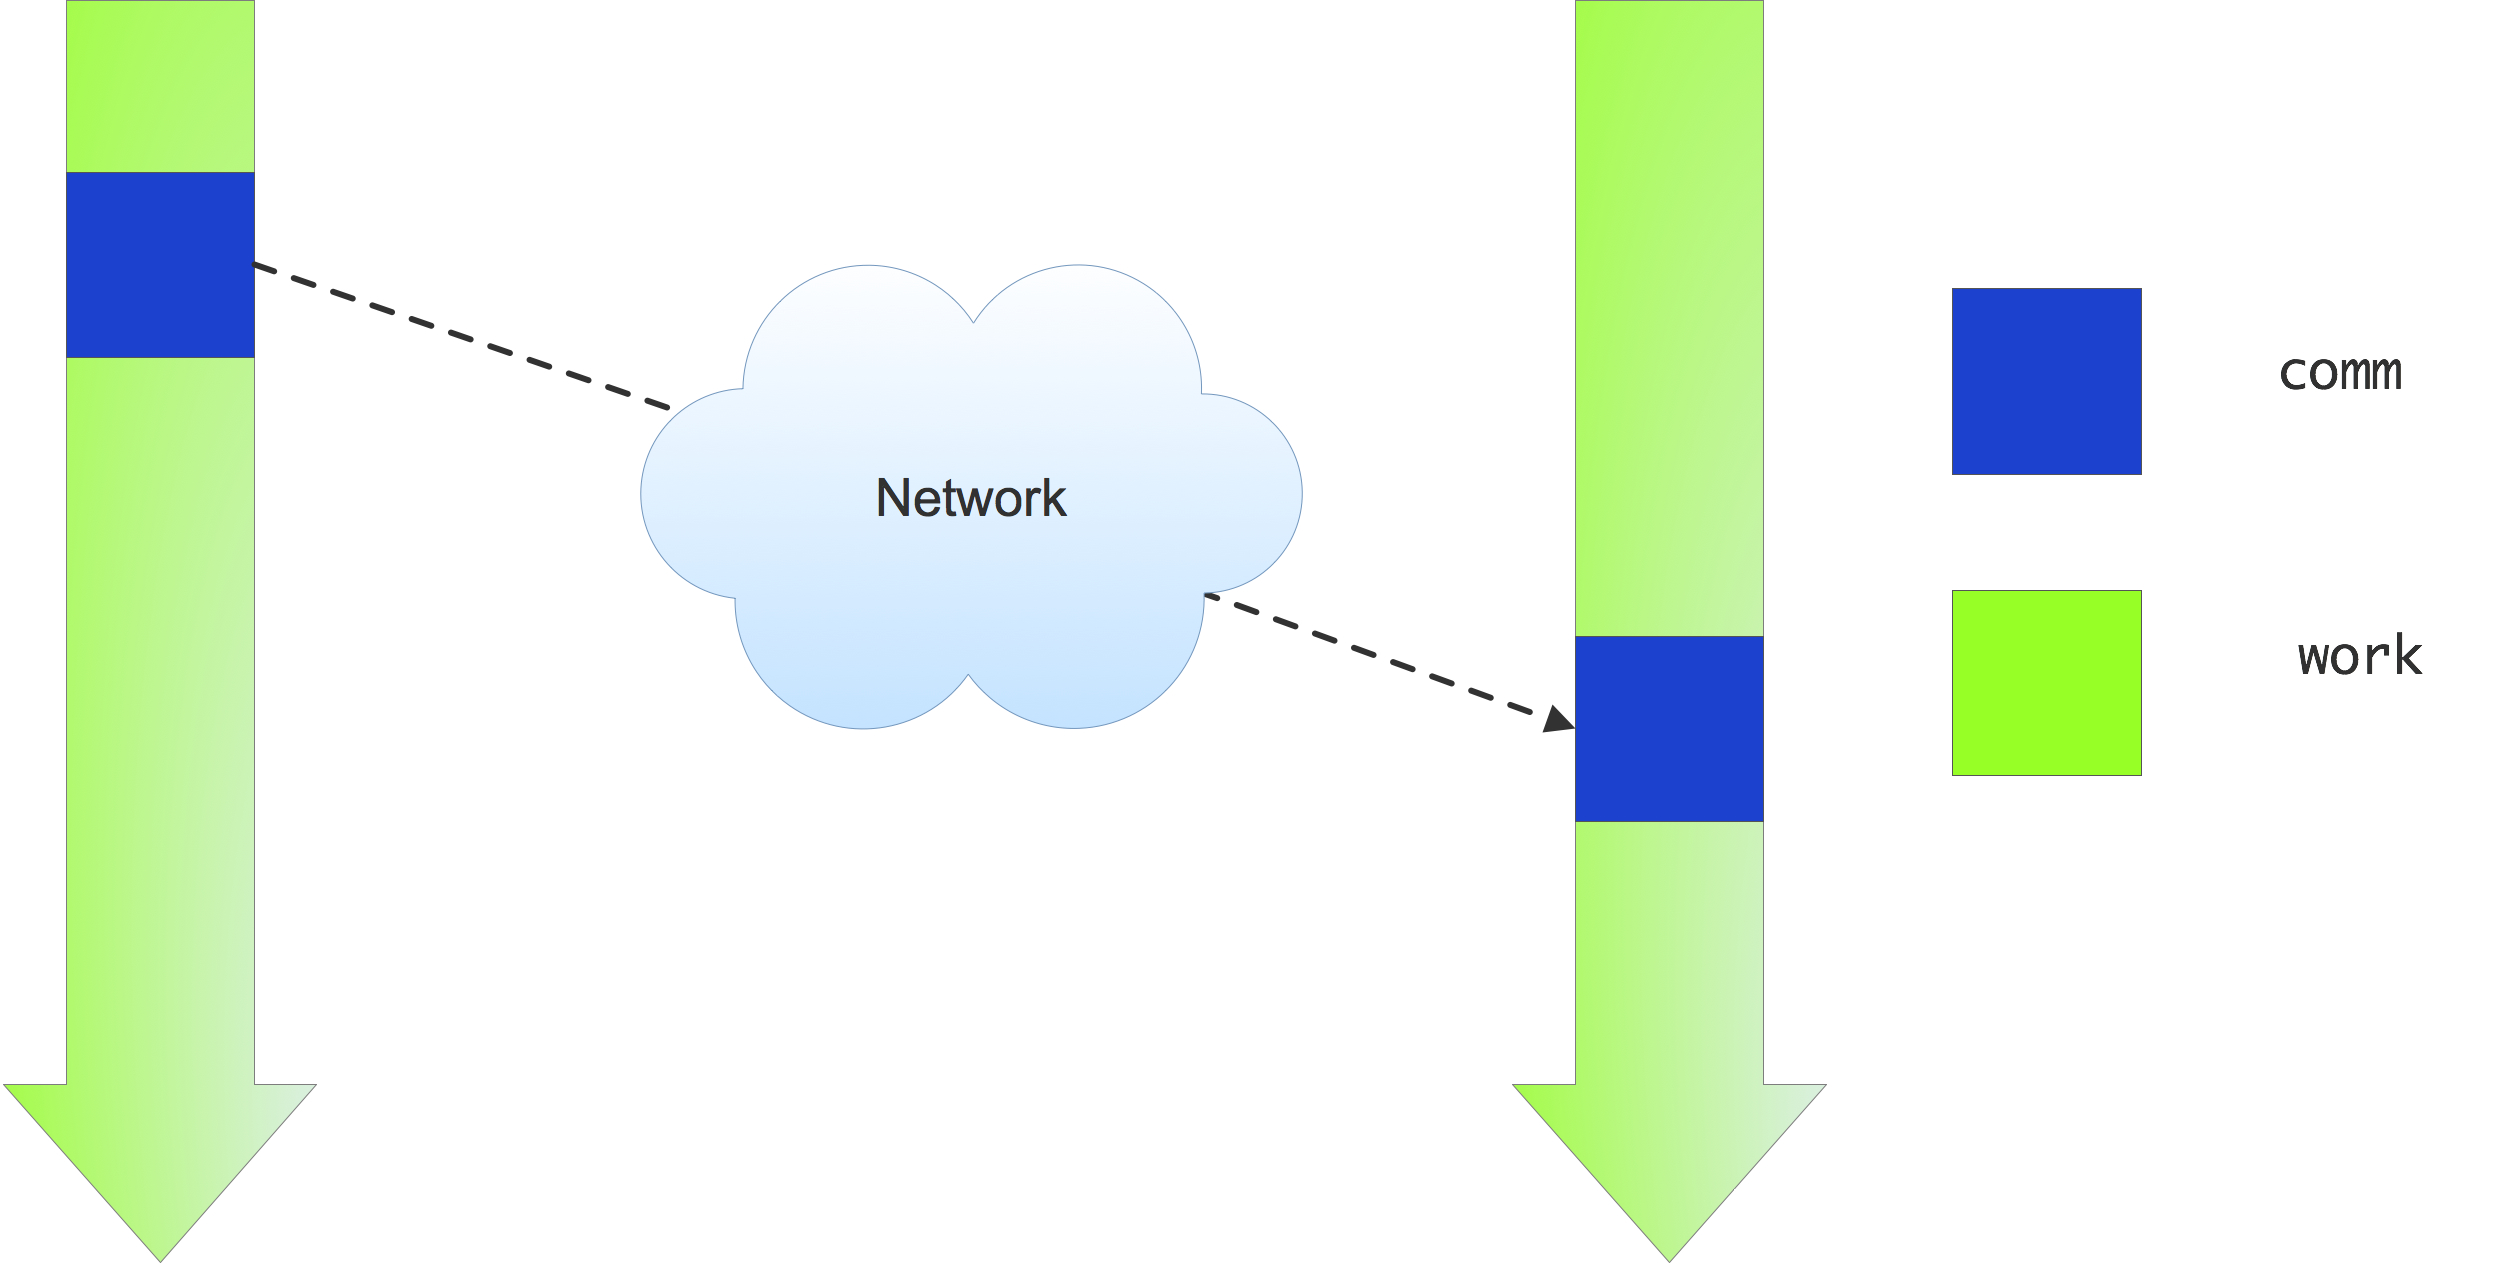
\includegraphics[scale=.07]{graphics/send-ideal}
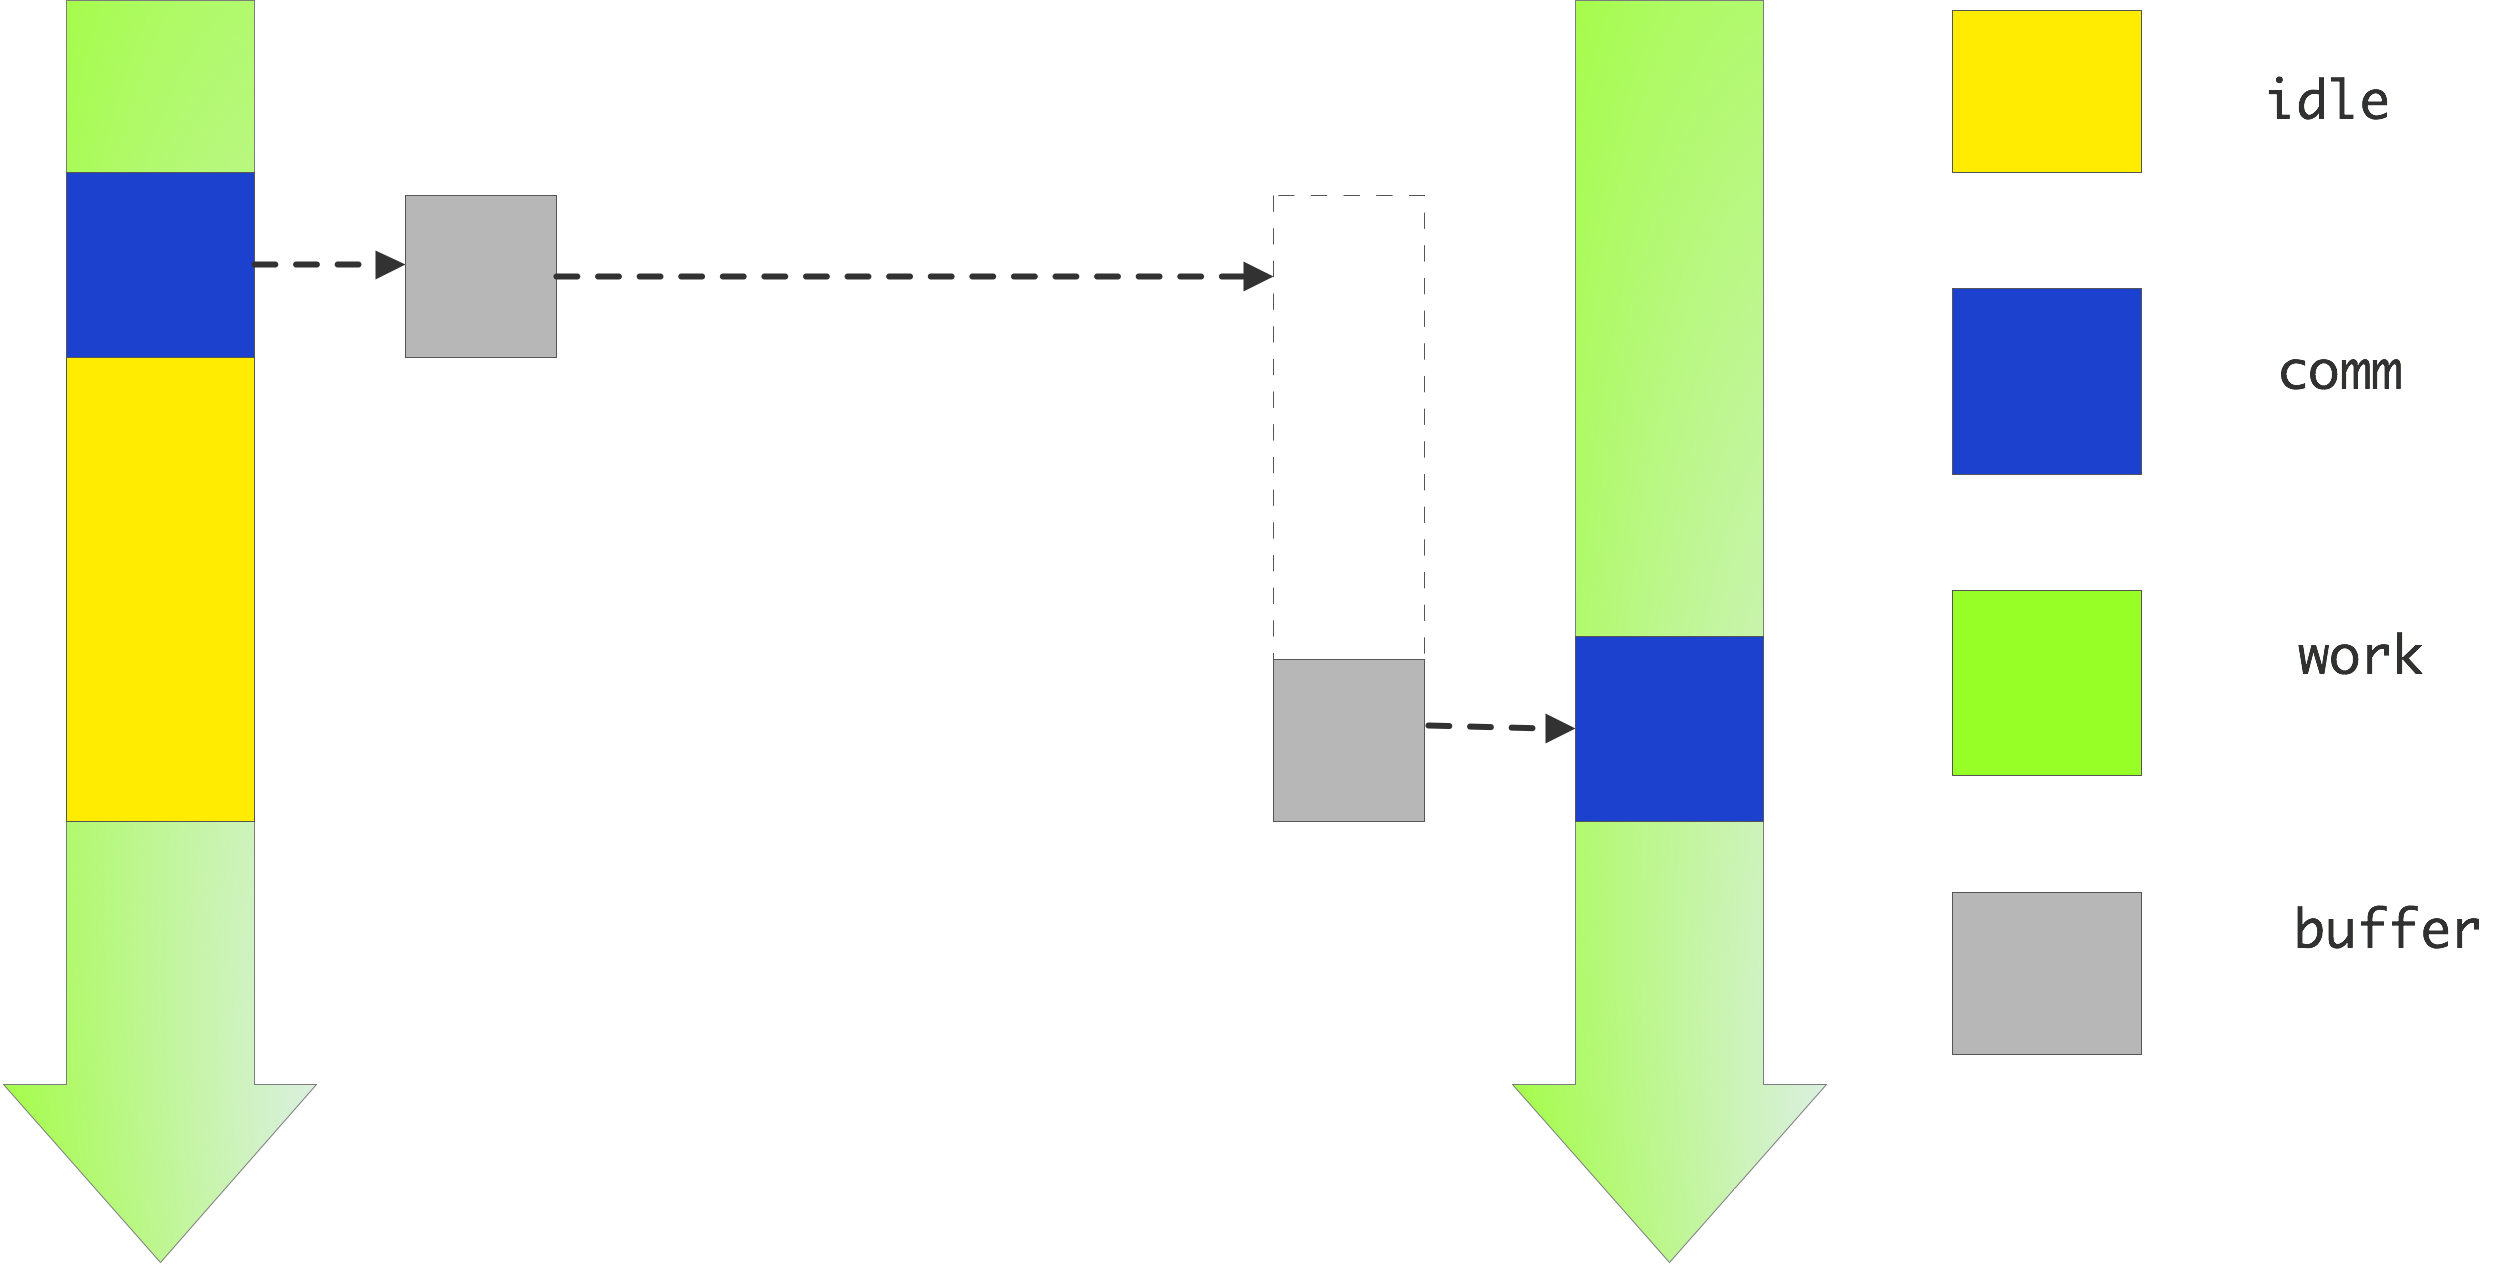
\includegraphics[scale=.07]{graphics/send-blocking}
}
Ideal vs actual send/recv behaviour.
\end{frame}

\begin{frame}[containsverbatim]\frametitle{Deadlock}
\lstset{language=C}
\begin{lstlisting}
other = 1-procno; /* if I am 0, other is 1; and vice versa */
receive(source=other);
send(target=other);
\end{lstlisting}

A subtlety.\\
This code may actually work:
\begin{lstlisting}
other = 1-procno; /* if I am 0, other is 1; and vice versa */
send(target=other);
receive(source=other);
\end{lstlisting}
Small messages get sent even if there is no corresponding receive.\\
(Often a system parameter)
\end{frame}


\begin{frame}{Protocol}
  \label{sl:rendezvous}
Communication is a `rendez-vous' or `hand-shake' protocol:
\begin{itemize}
\item Sender: `I have data for you'
\item Receiver: `I have a buffer ready, send it over'
\item Sender: `Ok, here it comes'
\item Receiver: `Got it.'
\end{itemize}
Small messages bypass this: `eager' send.\\
Definition of `small message' controlled by environment variables.
\end{frame}

\begin{exerciseframe}[serialsend]
  \input ex:serialsend
\end{exerciseframe}

\begin{frame}[containsverbatim]\frametitle{TAU trace: serialization}
  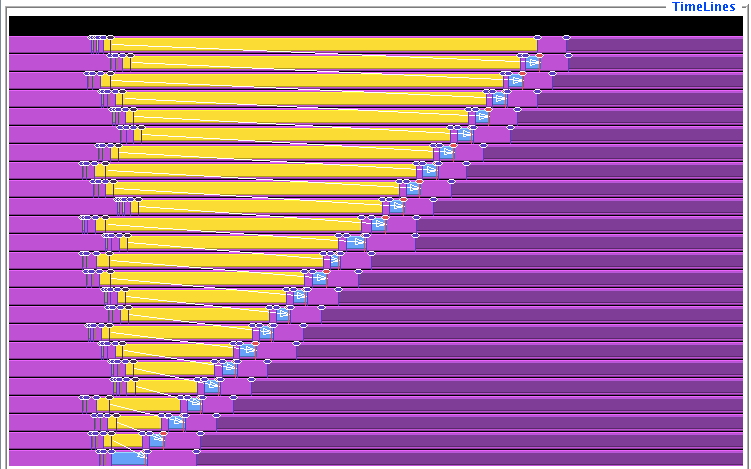
\includegraphics[scale=.4]{graphics/linear-serial}
  \label{fig:serialization}
\end{frame}

\begin{frame}{The problem here\ldots}
  Here you have a case of a program that computes the right output,\\
  just way too slow.

  Beware! Blocking sends/receives can be trouble. \\
  (How would you solve this particular case?)
\end{frame}

\begin{optexerciseframe}
  \input{ex:linear-sequential}
\end{optexerciseframe}

\sectionframe{Pairwise exchange}

\begin{frame}[containsverbatim]\frametitle{Operating on distributed data}
Take another look: \[ y_i=x_{i-1}+x_i+x_{i+1}\colon i=1,\ldots,N-1 \]

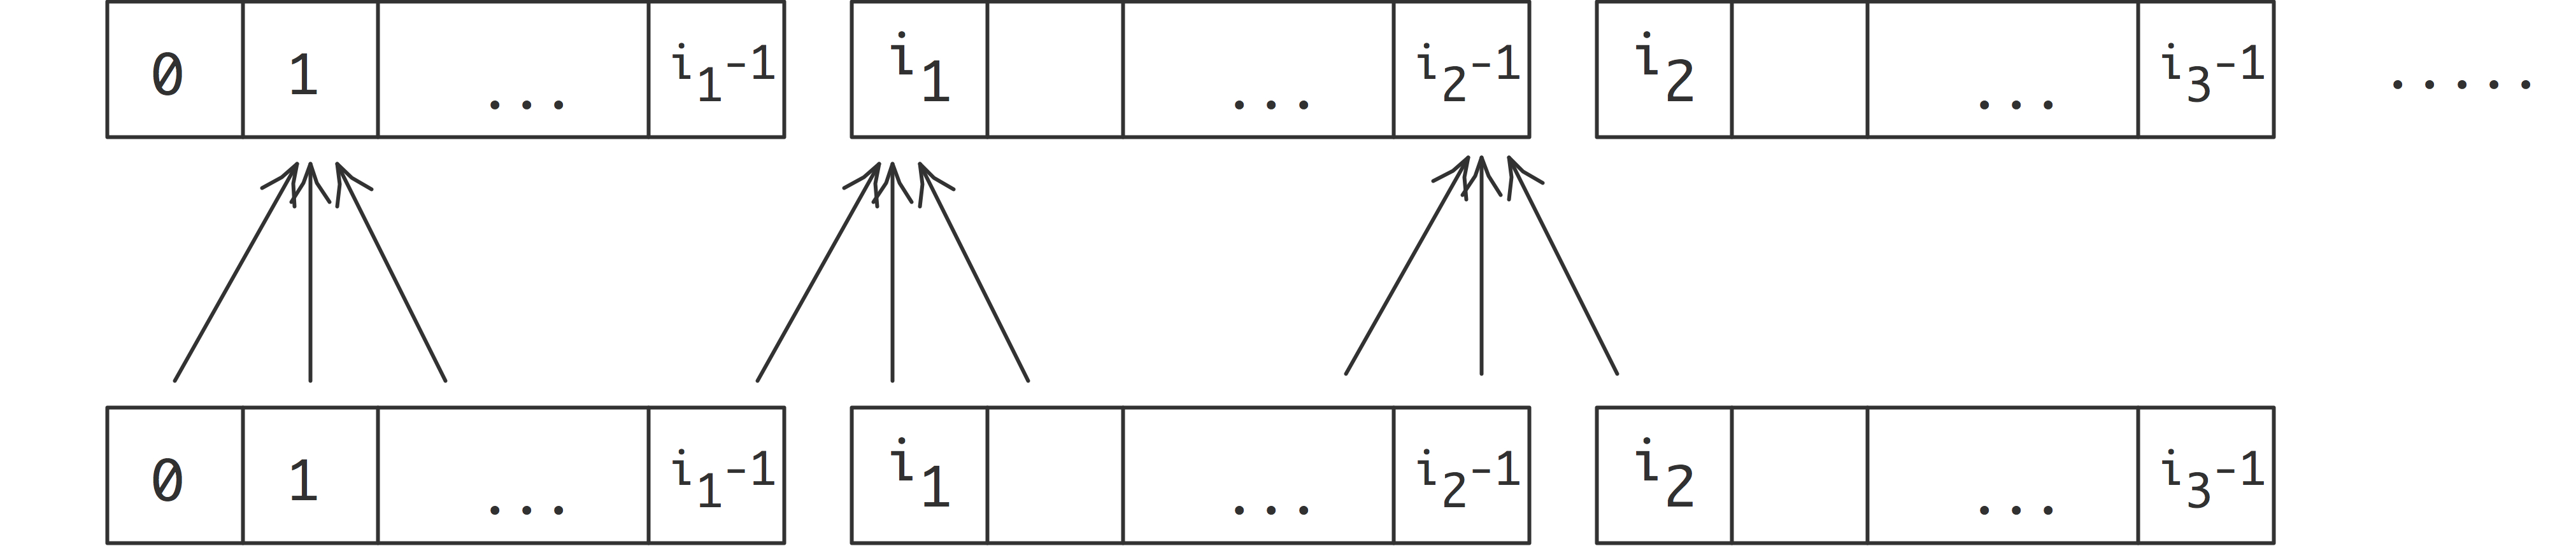
\includegraphics[scale=.09]{threepoint}

\begin{itemize}
\item One-dimensional data and linear process numbering;
\item Operation between neighbouring indices: communication between
  neighbouring processes.
\end{itemize}
\end{frame}

\begin{frame}{Two steps}
  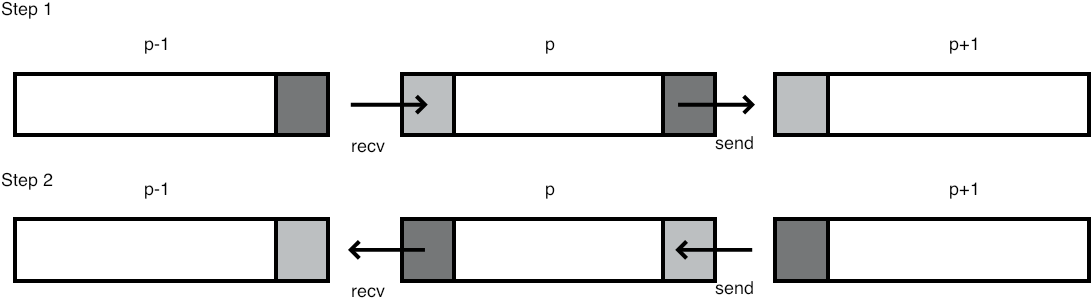
\includegraphics[scale=.2]{sendrecv-steps}

  First do all the data movement to the right, later to the left.
  \begin{itemize}
  \item Each process does a send and receive
  \item So everyone does the send, then the receive? We just saw the
    problem with that.
  \item Better solution coming up!
  \end{itemize}
\end{frame}

\begin{frame}[containsverbatim]\frametitle{Sendrecv}
  Instead of separate send and receive: use

  \lstinline{MPI_Sendrecv}

  Combined calling sequence of send and receive;\\
  execute such that no deadlock or sequentialization.
\end{frame}

\protoslide{MPI_Sendrecv}

\begin{frame}{SPMD picture}
  What does process $p$ do?
  
  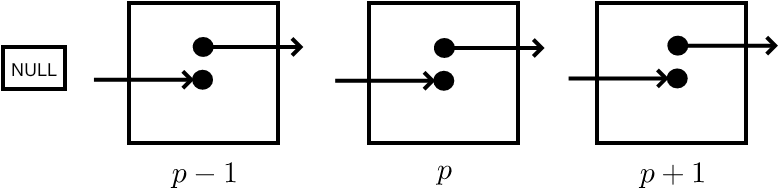
\includegraphics[scale=.4]{sendrecv-right}
\end{frame}

\begin{frame}[containsverbatim]\frametitle{Sendrecv with incomplete pairs}
\lstset{language=C}
\begin{lstlisting}
MPI_Comm_rank( .... &procno );
if ( /* I am not the first process */ )
  predecessor = procno-1;
else
  predecessor = MPI_PROC_NULL;

if ( /* I am not the last process */ )
  successor = procno+1;
else
  successor = MPI_PROC_NULL;

sendrecv(from=predecessor,to=successor);  
\end{lstlisting}
(Receive from \indexmpishow{MPI_PROC_NULL} succeeds without altering
the receive buffer.)
\end{frame}

\begin{frame}[containsverbatim]\frametitle{A point of programming style}
  The previous slide had:
  \begin{itemize}
  \item a conditional for computing the sender and receiver rank;
  \item a single Sendrecv call.
  \end{itemize}
  Also possible:
\lstset{language=C}
\begin{lstlisting}
if ( /* i am first */ )
  Sendrecv( to=right, from=NULL );
else if ( /* i am last */
  Sendrecv( to=NULL,  from=left );
else 
  Sendrecv( to=right, from=left );
\end{lstlisting}
But:\\
Code duplication is error-prone, also\\
chance of deadlock by missing a case
\end{frame}

\begin{optexerciseframe}[rightsend]
  \input ex:rightsendrecv
\end{optexerciseframe}

\begin{exerciseframe}[sendrecv]
  \input ex:3ptsendrecv
\end{exerciseframe}

\begin{frame}{Bucket brigade}
  Sometimes you really want to pass information from one process to
  the next: `bucket brigade'

  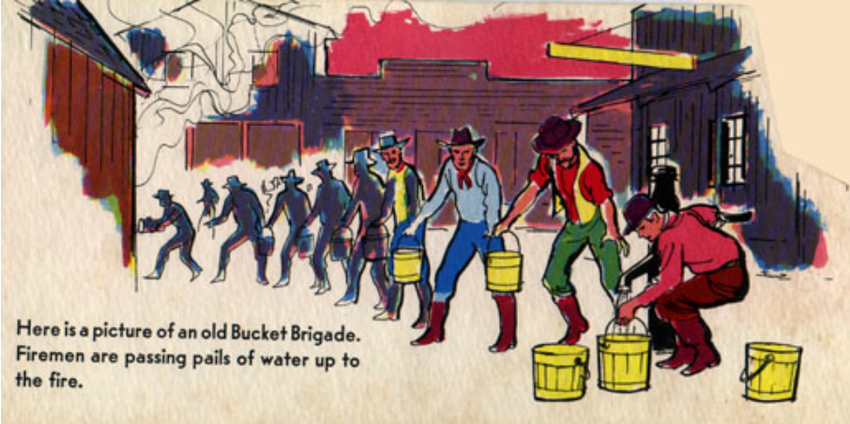
\includegraphics[scale=.4]{bucketbrigade}
\end{frame}

\begin{exerciseframe}[bucketblock]
  \input{ex:bucket-block}
\end{exerciseframe}

\begin{frame}{Odd-even transposition sort}
  \label{fig:swapsort1}

  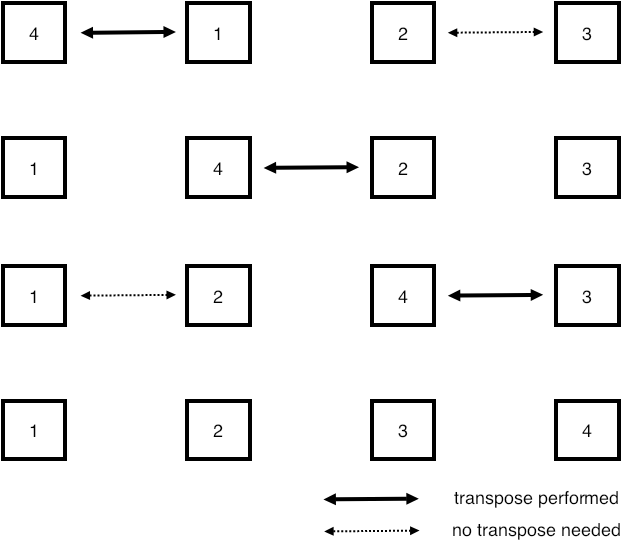
\includegraphics[scale=.3]{swapsort1}

  Odd-even transposition sort on 4 elements.
\end{frame}

\begin{optexerciseframe}
  \footnotesize
  %% \begin{wrapfigure}{r}{2.5in}
  %%   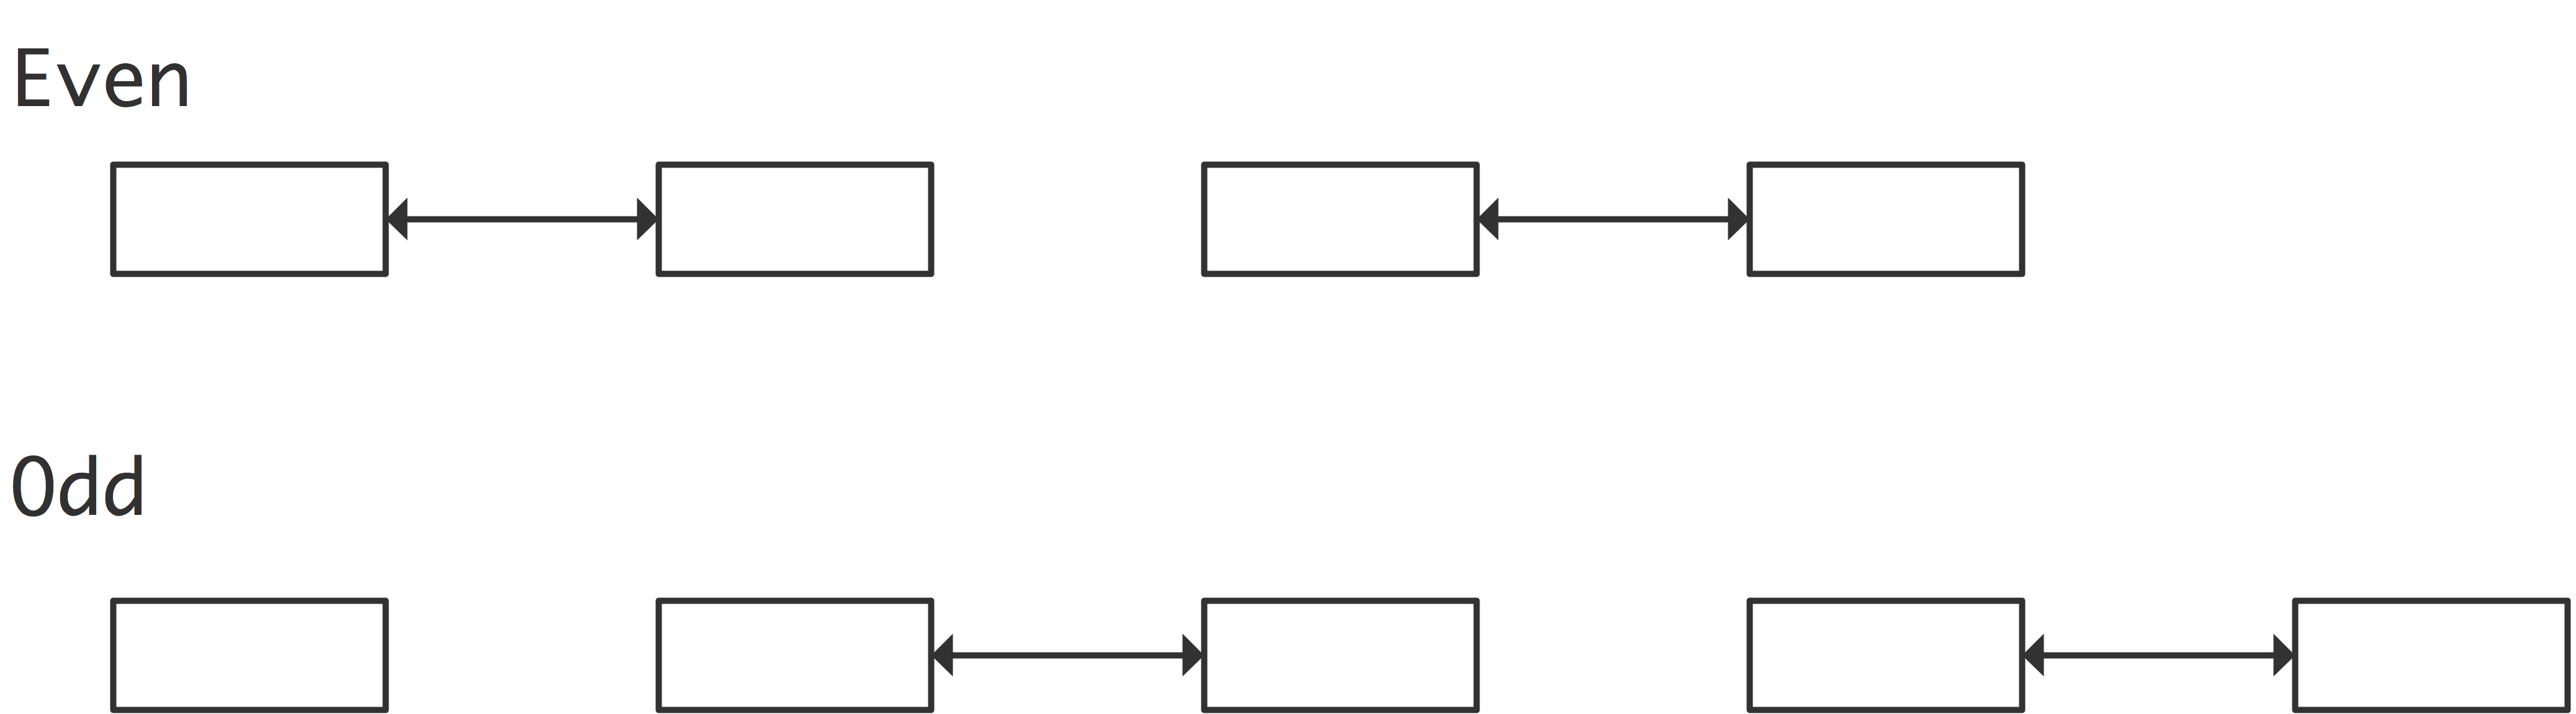
\includegraphics[scale=.04]{swapsort}
  %% \end{wrapfigure}
%
  \input ex:exchangesort
\end{optexerciseframe}

\sectionframe {Irregular exchanges: non-blocking communication}

\begin{frame}[containsverbatim]\frametitle{Sending with irregular connections}
  Graph operations:
  
  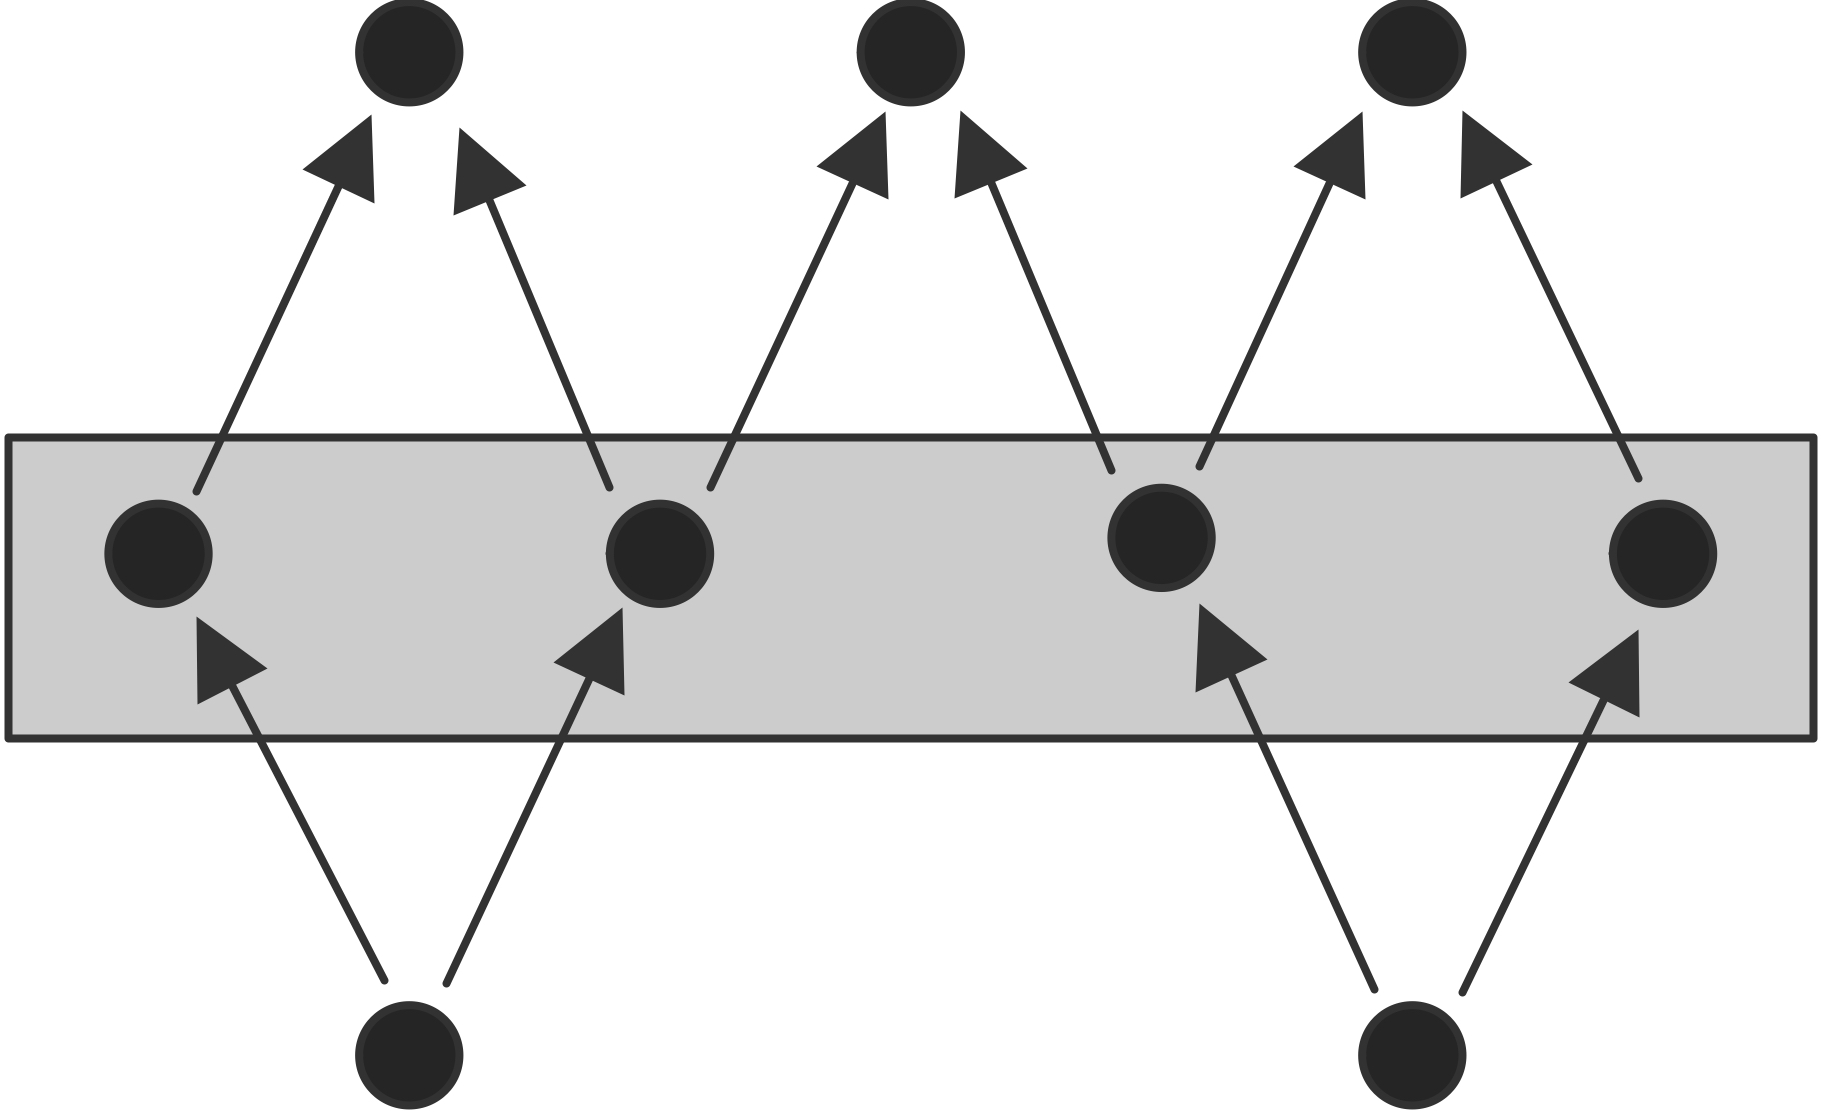
\includegraphics[scale=.1]{graphsend}
\end{frame}

\sectionframe{Communicating other than in pairs}
  
\begin{frame}{PDE, 2D case}
    A difference stencil applied to a two-dimensional square
    domain, distributed over processors. A cross-processor connection
    is indicated $\Rightarrow$ complicated to express pairwise

    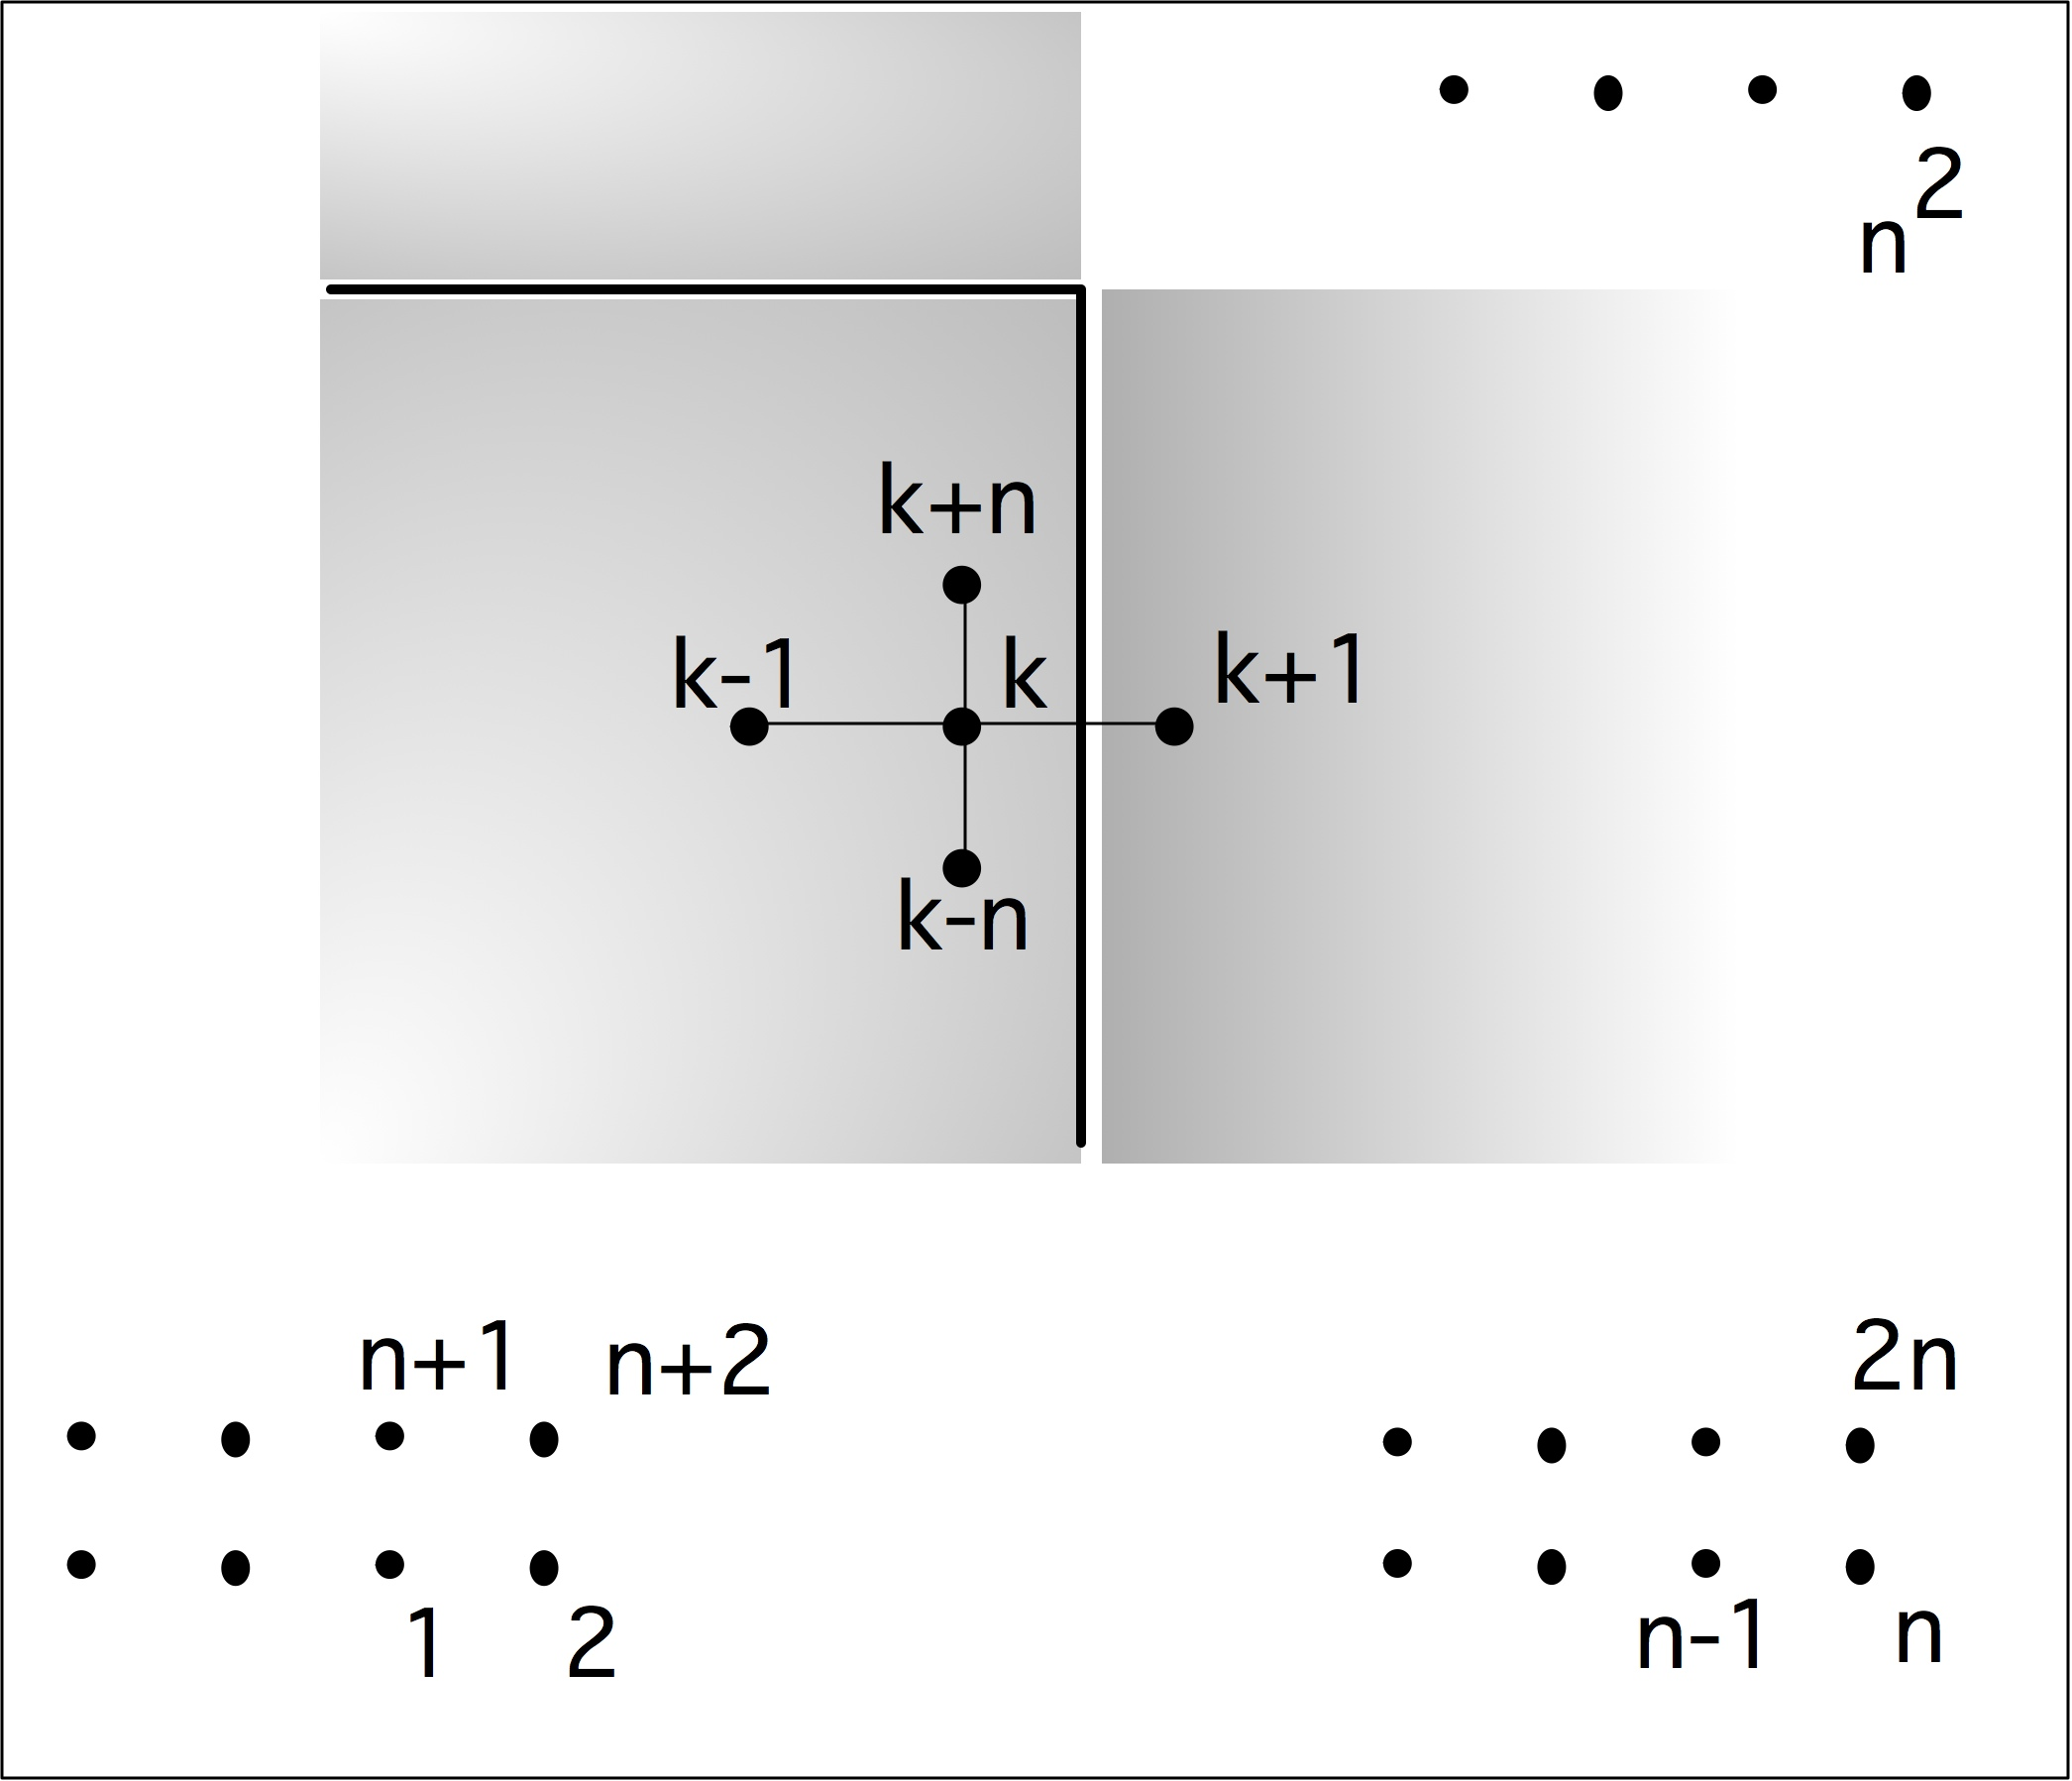
\includegraphics[scale=.1]{laplaceparallel}
\end{frame}

\begin{frame}{Halo region}
  The halo region of a process, induced by a stencil

  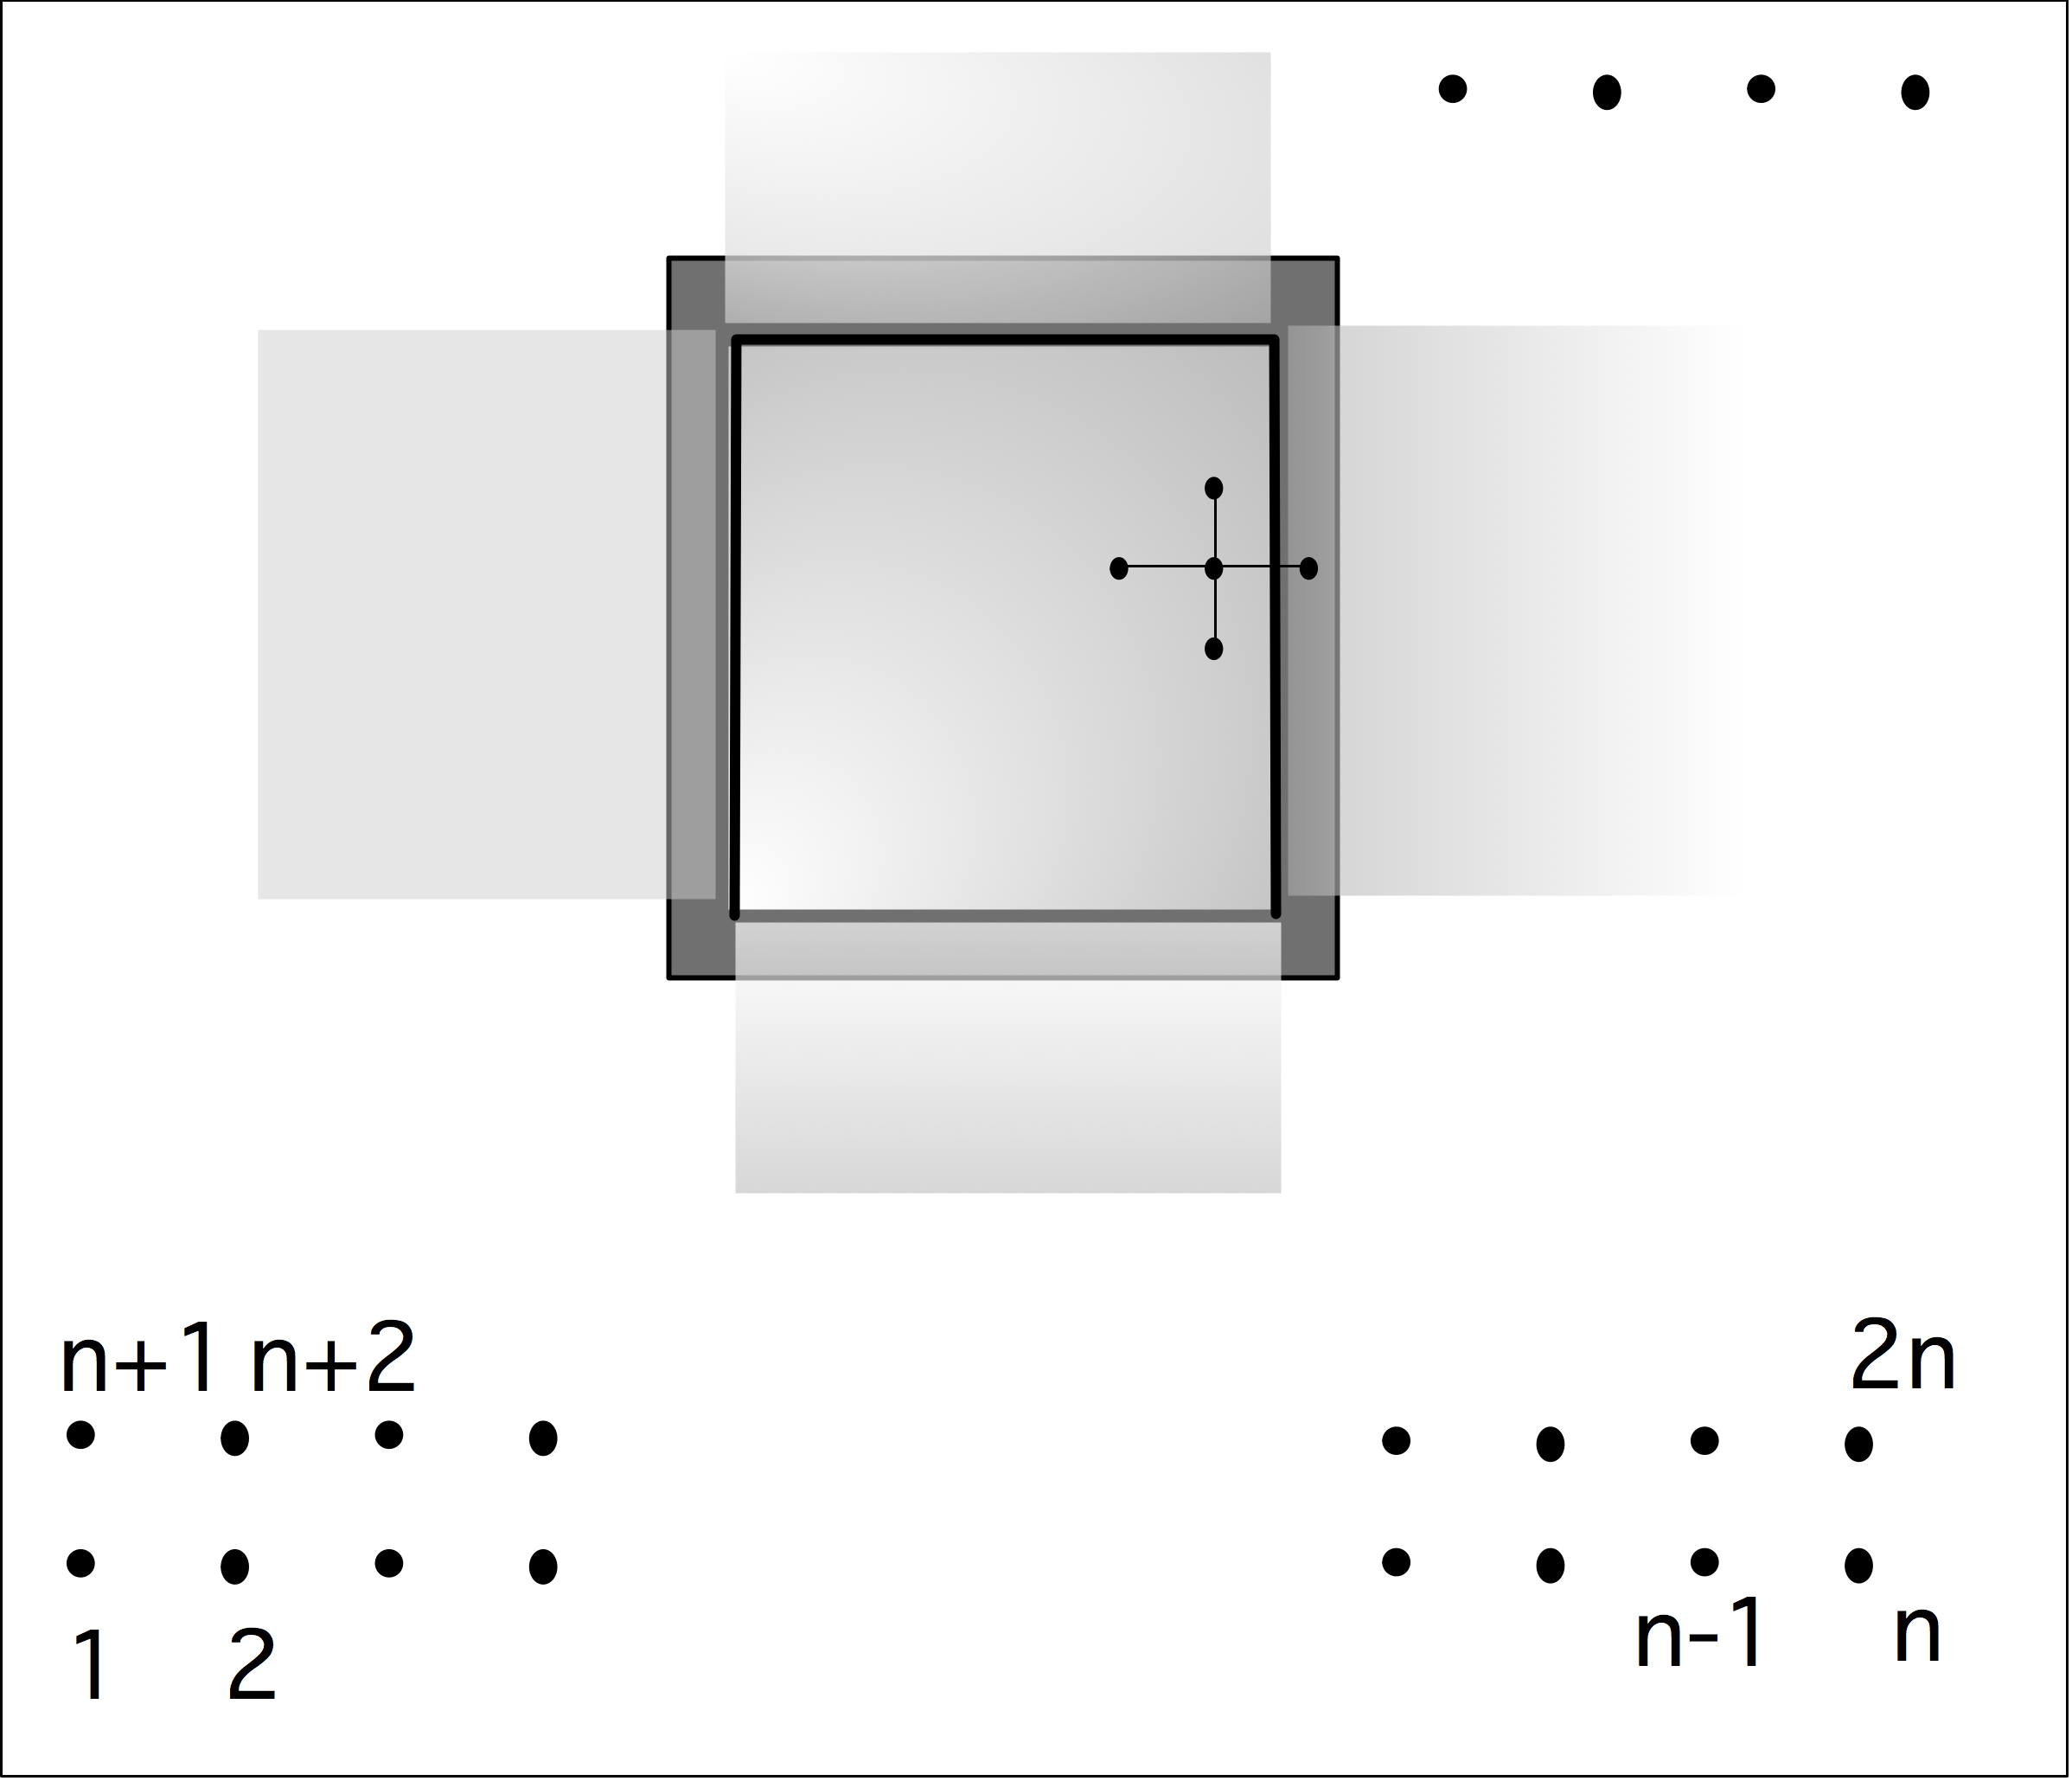
\includegraphics[scale=.1]{laplaceghost}
\end{frame}

\begin{frame}{PDE matrix}
  \footnotesize
  \[
    A=
    \left(\begin{array}{ccccc|ccccc|cc}
      4&-1&&&\emptyset&-1&&&&\emptyset&\\ 
      -1&4&-1&&&&-1&&&&\\ 
      &\ddots&\ddots&\ddots&&&&\ddots&&\\ 
      &&\ddots&\ddots&-1&&&&\ddots&\\ 
      \emptyset&&&-1&4&\emptyset&&&&-1&\\ \hline
      -1&&&&\emptyset&4&-1&&&&-1\\
      &-1      &      &&&-1      &4       &-1      &&&&-1\\
      &\uparrow&\ddots&&&\uparrow&\uparrow&\uparrow&&  &&\uparrow\\
      &k-n     &      &&&k-1     &k       &k+1     &&-1&&k+n\\
      &&&&-1&&&&-1&4&&\\ \hline
      &        &      &&&\ddots  &        &        &&  &\ddots\\
    \end{array}\right)
    \]
\end{frame}

\begin{frame}[containsverbatim]\frametitle{How do you approach this?}
  \begin{itemize}
  \item It is very hard to figure out a send/receive sequence that
    does not deadlock or serialize
  \item Even if you manage that, you may have process idle time.
  \end{itemize}
  Instead: 
  \begin{itemize}
  \item Declare `this data needs to be sent' or `these messages are expected', and
  \item then wait for them collectively.
  \end{itemize}
\end{frame}

\begin{frame}[containsverbatim]\frametitle{Non-blocking send/recv}
\lstset{language=C}
\begin{lstlisting}
// start non-blocking communication
MPI_Isend( ... ); MPI_Irecv( ... );
// wait for the Isend/Irecv calls to finish in any order
MPI_Wait( ... );  
\end{lstlisting}
\end{frame}

\begin{frame}[containsverbatim]\frametitle{Syntax}
  \small
  Very much like blocking \indexmpishow{MPI_Send}/\indexmpishow{MPI_Recv}:
\lstset{language=C}
\begin{lstlisting}
int MPI_Isend(void *buf,
  int count, MPI_Datatype datatype, int dest, int tag,
  MPI_Comm comm, MPI_Request *request)
int MPI_Irecv(void *buf,
  int count, MPI_Datatype datatype, int source, int tag,
  MPI_Comm comm, MPI_Request *request)  
\end{lstlisting}
The \indexmpishow{MPI_Request}s can be tested:
\begin{lstlisting}
int MPI_Waitall(int count, MPI_Request array_of_requests[], 
  MPI_Status array_of_statuses[])
\end{lstlisting}
\begin{itemize}
\item ignore status: \indexmpishow{MPI_STATUSES_IGNORE}
\item also \indexmpishow{MPI_Wait}, \indexmpishow{MPI_Waitany}, \indexmpishow{MPI_Waitsome}
\end{itemize}
\end{frame}

\begin{exerciseframe}[isendirecv]
  \input ex:3ptnonblock
  
  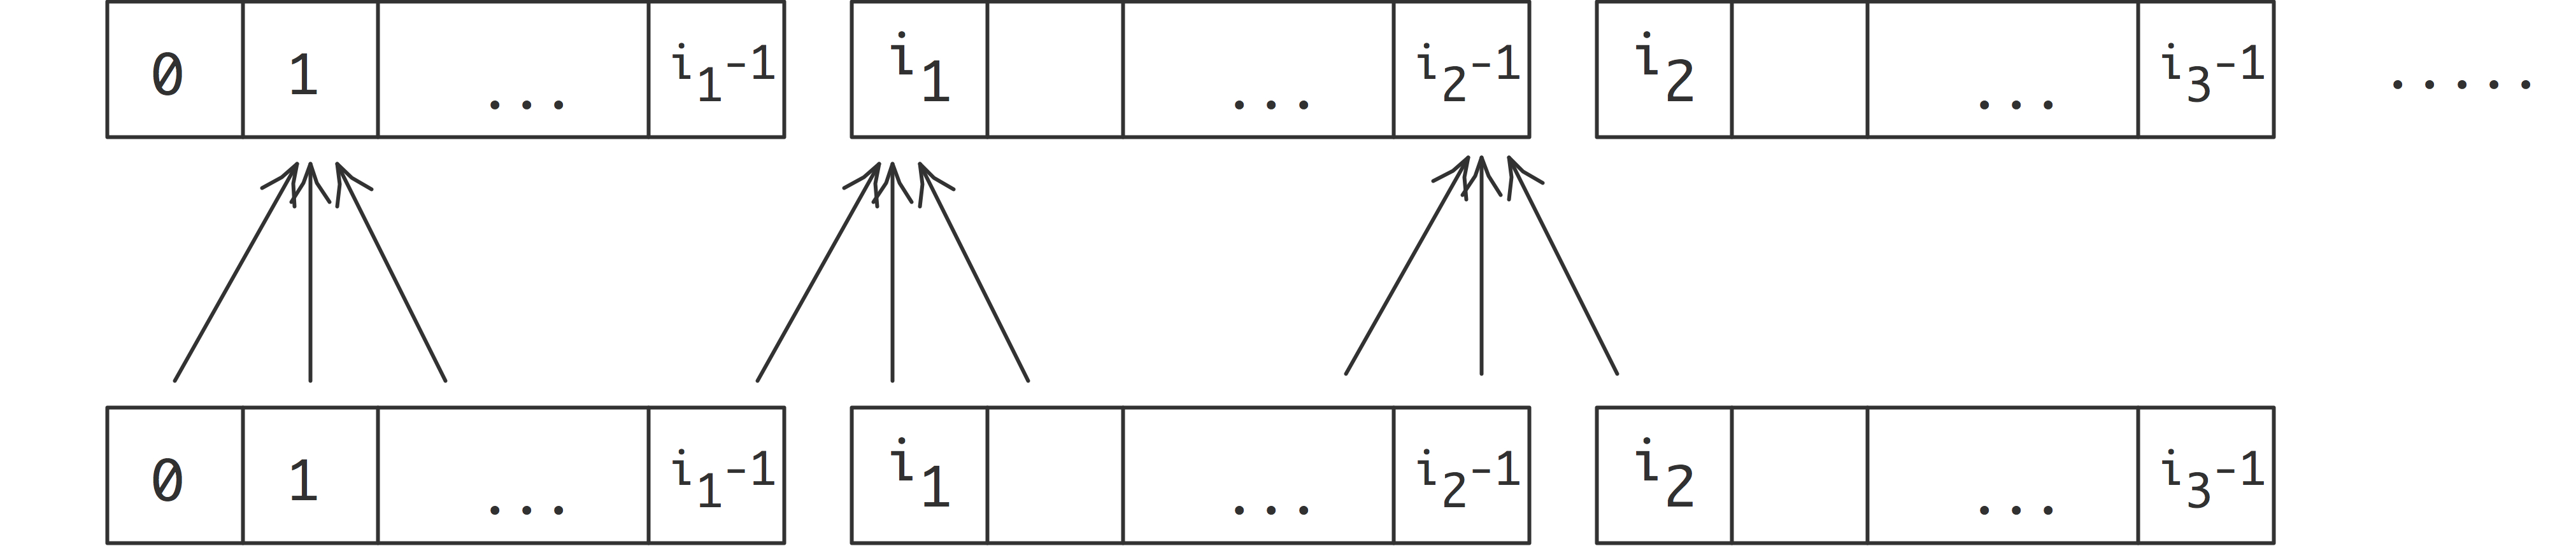
\includegraphics[scale=.08]{threepoint}

  (Can you think of a different way of handling the end points?)
\end{exerciseframe}

\begin{frame}[containsverbatim]\frametitle{Comparison}
  \begin{itemize}
  \item Obvious: blocking vs non-blocking behaviour.
  \item Buffer reuse: when a blocking call returns, the buffer
    is safe for reuse;
  \item A buffer in a non-blocking call can only be reused
    after the wait call.
  \end{itemize}
\end{frame}

\begin{frame}[containsverbatim]\frametitle{Buffer use in blocking/non-blocking case}
Blocking:
\lstset{language=C}
\begin{lstlisting}
double *buffer;
for ( ... p ... ) {
   buffer = // fill in the data
   MPI_Send( buffer, ... /* to: */ p );
\end{lstlisting}
Non-blocking:
\begin{lstlisting}
double **buffers;
for ( ... p ... ) {
   buffers[p] = // fill in the data
   MPI_Isend( buffers[p], ... /* to: */ p );
\end{lstlisting}
\end{frame}

\begin{frame}[containsverbatim]\frametitle{Latency hiding}
  Other motivation for non-blocking calls:\\
  overlap of computation and communication, provided
  hardware support.

  Also known as `latency hiding'.

  Example: three-point combination operation (see above):
  \begin{enumerate}
  \item Start communication for edge points,
  \item Do local operations while communication goes on,
  \item Wait for edge points from neighbour processes
  \item Incorporate incoming data.
  \end{enumerate}
\end{frame}

\begin{frame}{Matrices in parallel}
  \[ y\leftarrow Ax\]
  and $A,x,y$ all distributed:

  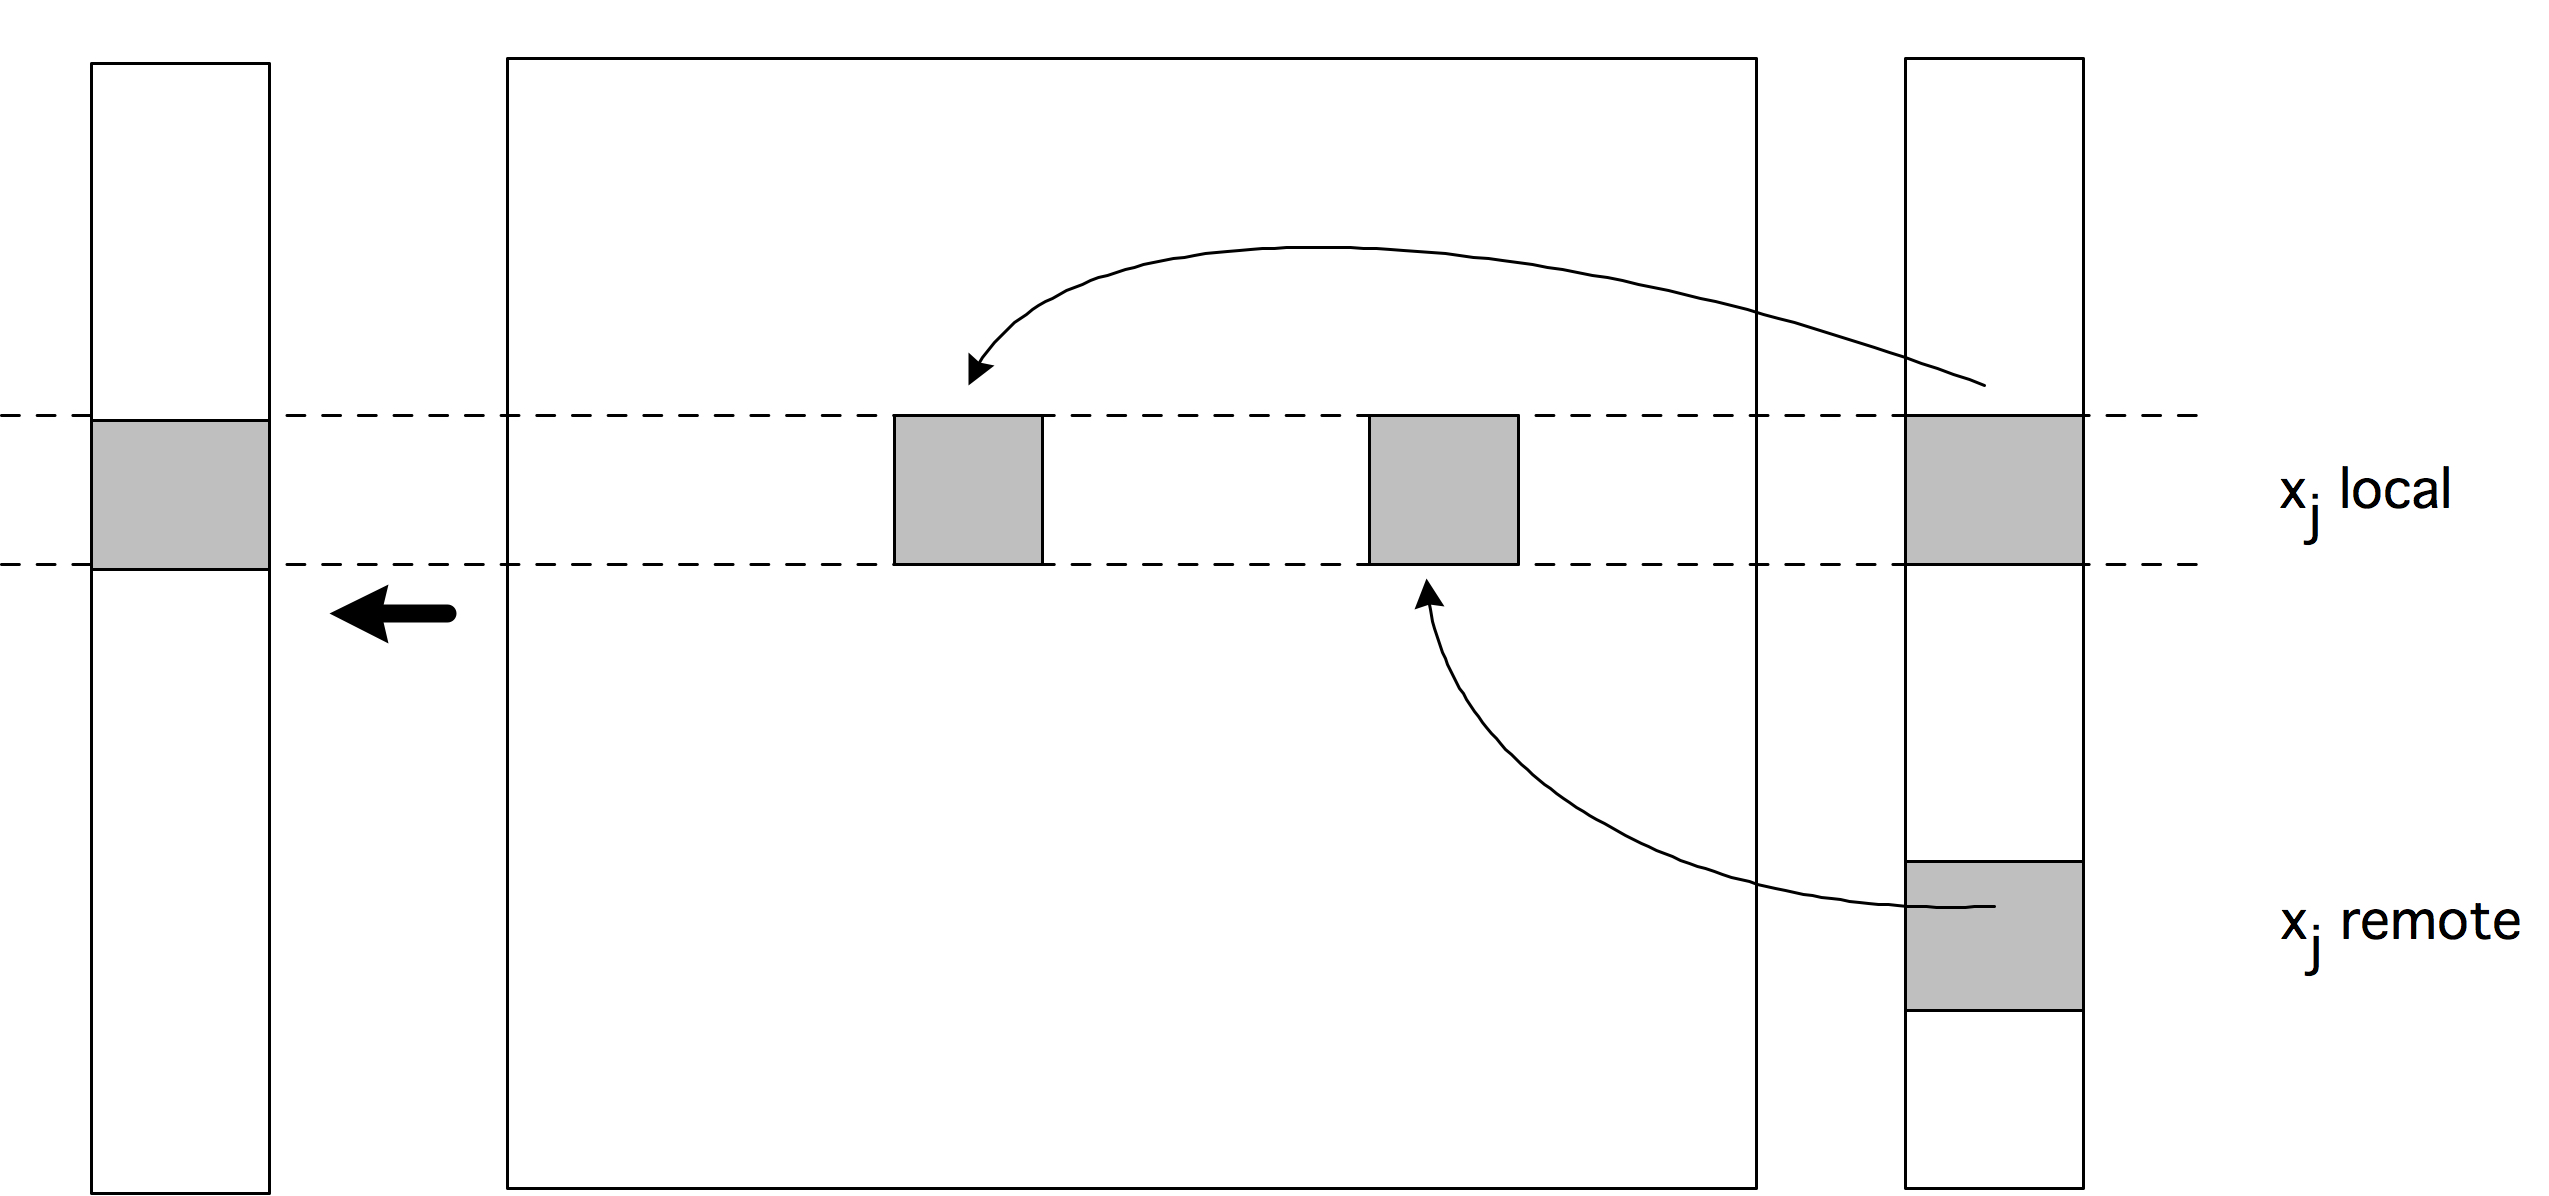
\includegraphics[scale=.12]{distmvp}
\end{frame}

\begin{frame}{Hiding the halo}
  Interior of a process domain can overlap with halo transfer:

  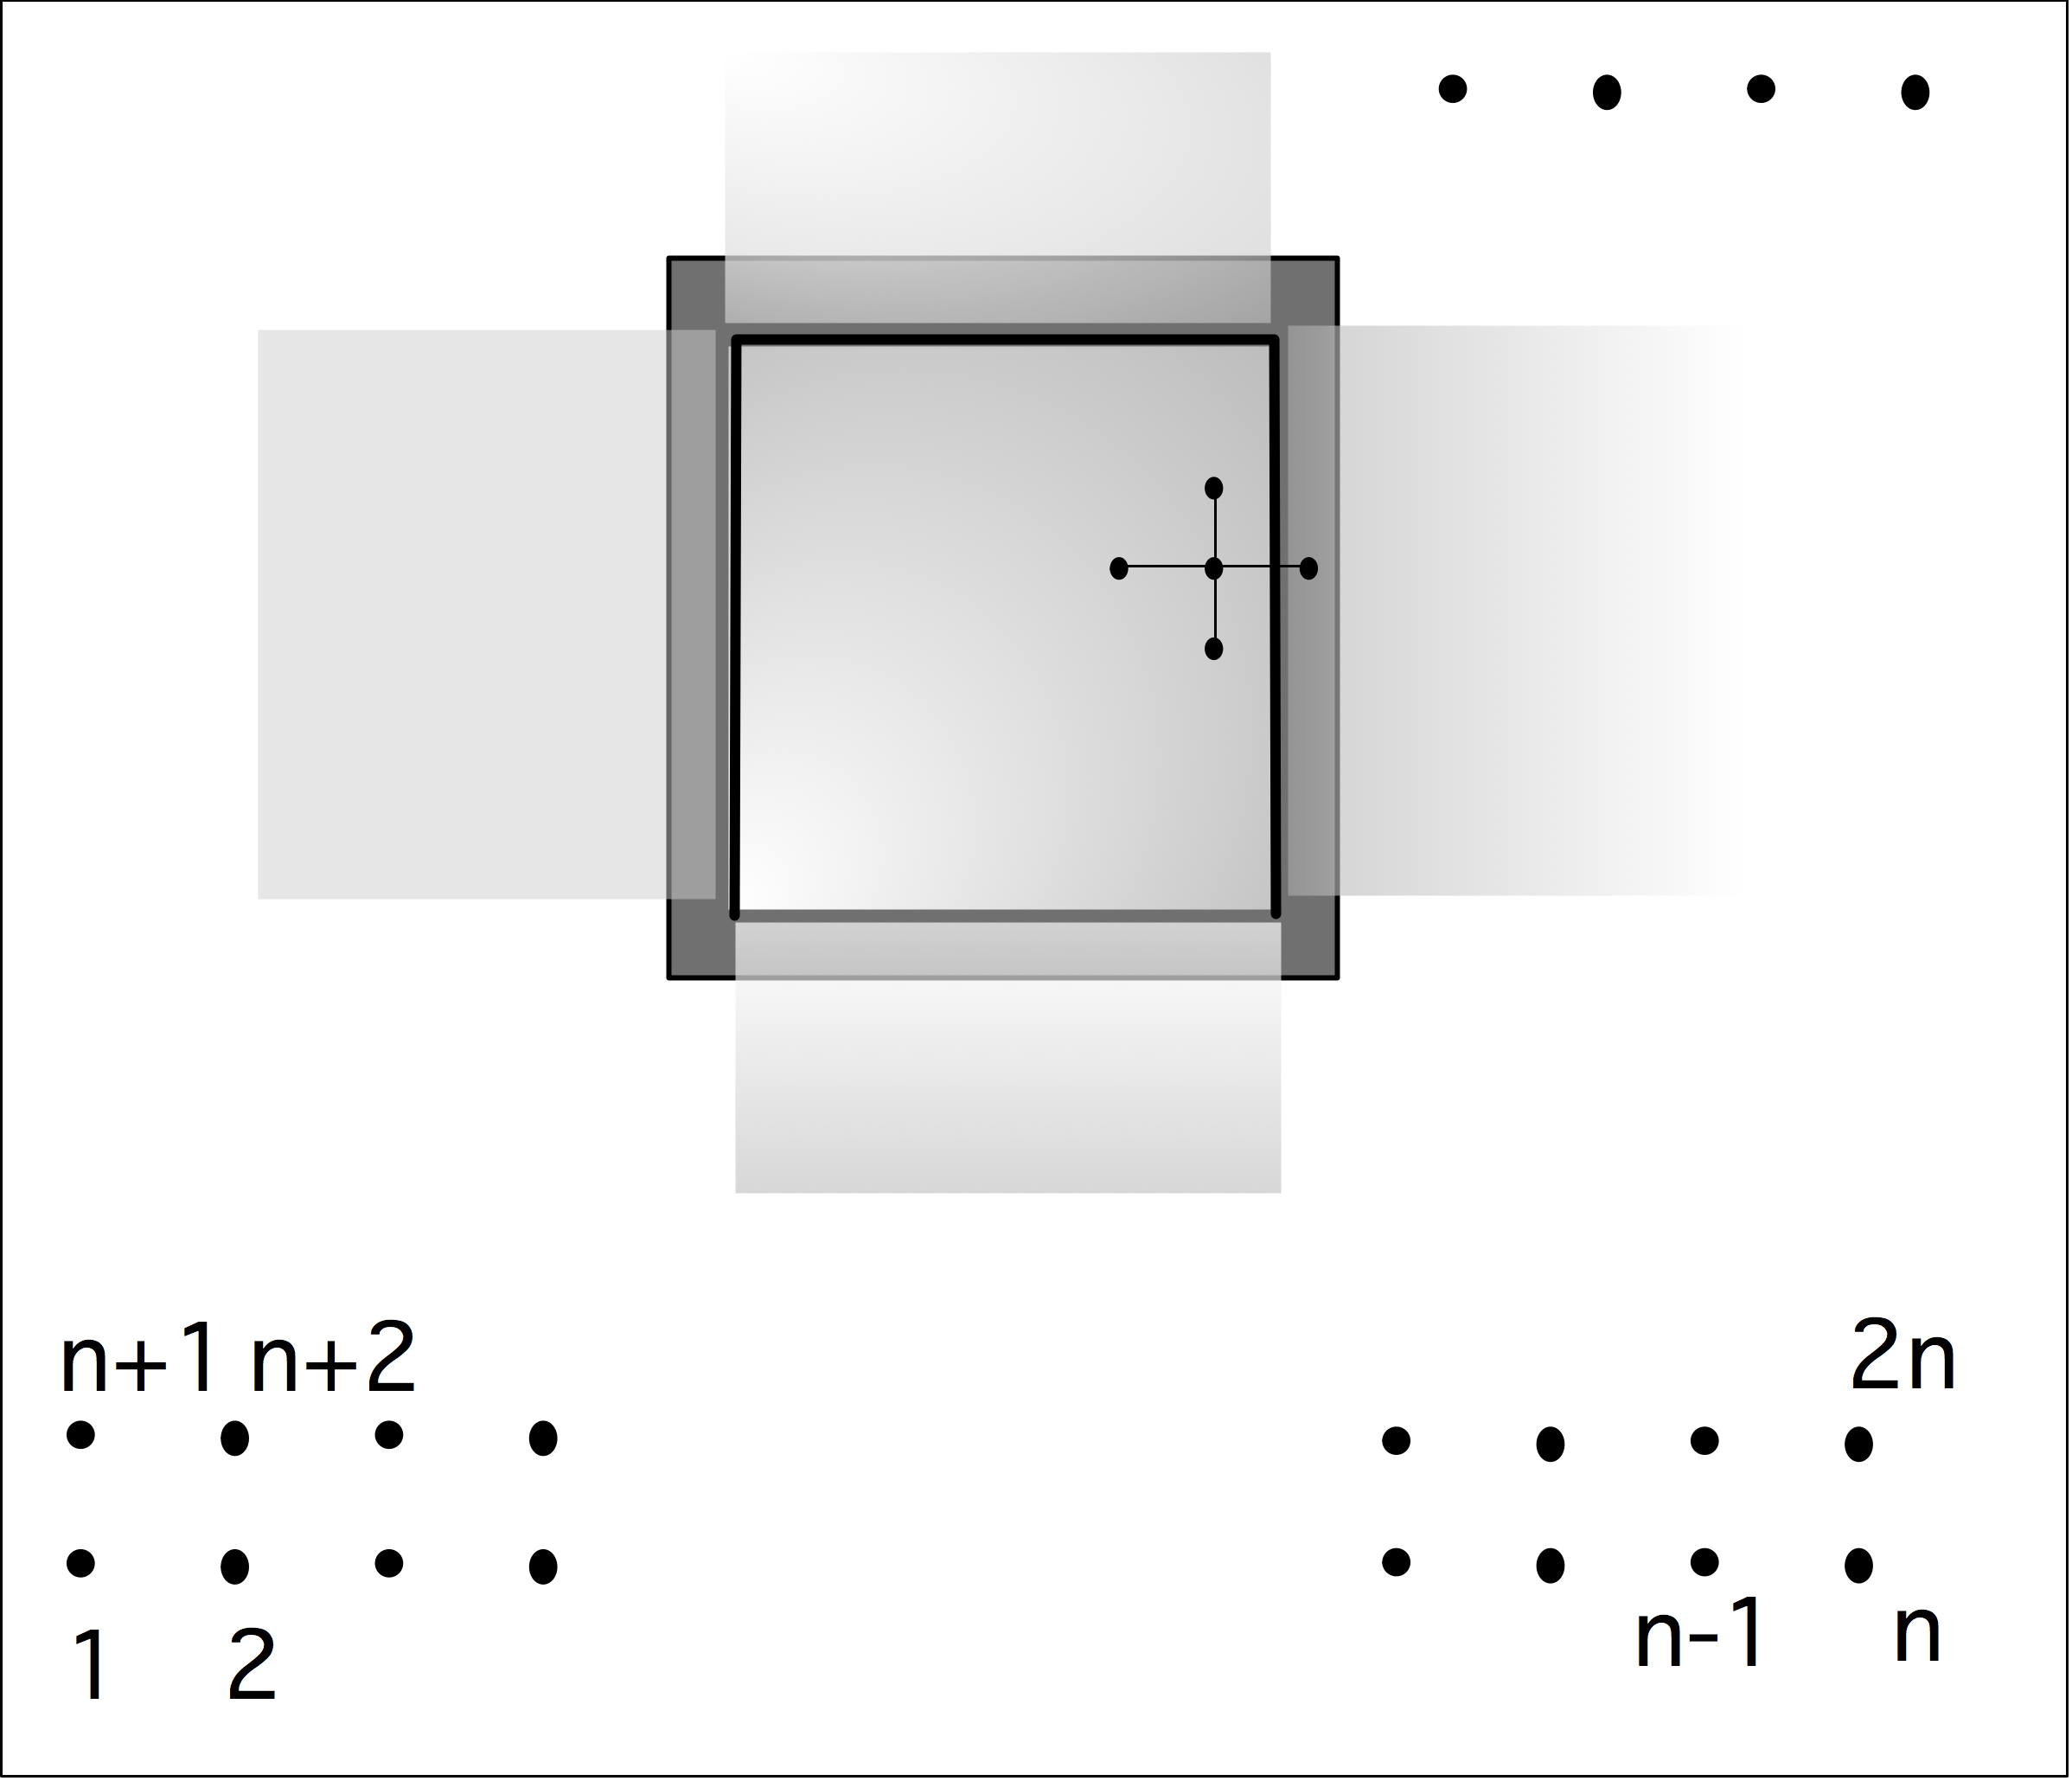
\includegraphics[scale=.1]{laplaceghost}
\end{frame}

\begin{exerciseframe}[isendirecvarray]
  \input ex:3ptnonblock-hide

  Write your code so that it can achieve latency hiding.
\end{exerciseframe}

\begin{frame}[containsverbatim]\frametitle{Test: non-blocking wait}
  \begin{itemize}
  \item Post non-blocking receives
  \item test for incoming messages
  \item if nothing comes in, do local work
  \end{itemize}
\lstset{language=C}
\begin{lstlisting}
while (1) {
  MPI_Test( /* from: */ MPI_ANY_SOURCE, &flag );
  if (flag)
    // do something with incoming message
  else
    // do local work
}
\end{lstlisting}
\end{frame}

\begin{frame}[containsverbatim]{The Pipeline Pattern}
  \begin{itemize}
  \item Remember the bucket brigade: data propagating through
    processes
  \item If you have many buckets being passed: pipeline
  \item This is very parallel: only filling and draining the pipeline
    is not completely parallel
  \item Application to long-vector broadcast: pipelining gives overlap
  \end{itemize}
\end{frame}

\begin{optexerciseframe}[bucketpipenonblock]
  Implement a pipelined broadcast for long vectors:\\
  use non-blocking communication to send the vector in parts.
\end{optexerciseframe}

\begin{frame}[containsverbatim]\frametitle{More sends and receive}
  \begin{itemize}
  \item \indexmpishow{MPI_Bsend}, \indexmpishow{MPI_Ibsend}: buffered send
  \item \indexmpishow{MPI_Ssend}, \indexmpishow{MPI_Issend}: synchronous send
  \item \indexmpishow{MPI_Rsend}, \indexmpishow{MPI_Irsend}: ready send
  \item Persistent communication: repeated instance of same proc/data description.
  \end{itemize}
  too obscure to go into.
\end{frame}

\endinput

\begin{frame}[containsverbatim]\frametitle{}
\begin{lstlisting}
  
\end{lstlisting}
\end{frame}

